\section{Experimental setup\label{sec:setup}}

\subsection{Motivation\label{sec:setup-motivation}}

Radiation damage in plastic scintillators causes a loss in light output that depends exponentially on the integrated dose. The light output L(\textit{d}) after an integrated dose \textit{d} is expressed in the following equation:

\begin{equation}
L(\textit{d}) = L(0)\cdot e^{-d/D(\textit{r})}
\label{eq:lightloss}
\end{equation}

where the exponential function is characterized by a dose constant D(\textit{r}) that depends on factors such as dose rate \textit{r}, material composition of the scintillator, and the presence of oxygen in and around the scintillator material. The dependence of D(\textit{r}) on these various factors is still under study; references to past and ongoing studies can be found here (\textbf{insert list of references}).

The goals of the present study are:

\begin{itemize}
\item To measure the dose constant D(r) for SCSN81 (the type currently used in the CMS HCAL detector), and compare its consistency with measurements from other experiments.
\item To measure the dose constant D(r) for various candidate materials for future upgrades to the CMS HCAL, in order to assess how their radiation tolerance compares to that of SCSN81.
\item To test the operational stability of Phase I HCAL endcap (HE) readout electronics in the CMS cavern.
\end{itemize}

\subsection{Scintillator tiles\label{sec:setup-tiles}}

Apart from a few special tile geometries that will be described at the end of this section, most of the plastics scintillator tiles used in this study come in one of two shapes: sigma tiles or finger tiles.

Sigma tiles have dimensions 10 cm $\times$ 10 cm $\times$ 3.7 mm. A wavelength-shifting (WLS) fiber enters at a hole in one corner of the square and passes through a groove that follows the perimeter of the square in a sigma-shaped trajectory until it reaches the same corner where it entered the tile. The total length of the WLS fiber, including the part sticking out of the tile, is roughly 52 cm. During the experiment, ultraviolet laser light is shined onto a small point at the center of the square tile (i.e., only onto the tile material and not onto the WLS fiber), and the scintillation light produced by the tile material is collected by the WLS fiber.

Finger tiles have dimensions 10 cm $\times$ 2 cm $\times$ 3.7 mm. A WLS fiber enters the tile at the center of one of the short ends of the rectangle and passes through a groove that runs straight along the length of the tile. The total length of the WLS fiber, including the part sticking out of the tile, is roughly 20 cm. Ultraviolet laser light is shined onto a point at the center of the rectangle, illuminating both the tile material and the WLS fiber, but the excitation of the WLS fiber is considered negligible in this experiment. The scintillation light from the tile is collected by the WLS fiber. Figure~\ref{fig:sigma-finger} shows pictures of a sigma tile and a finger tile.

\begin{figure}[hbtp]
\begin{center}
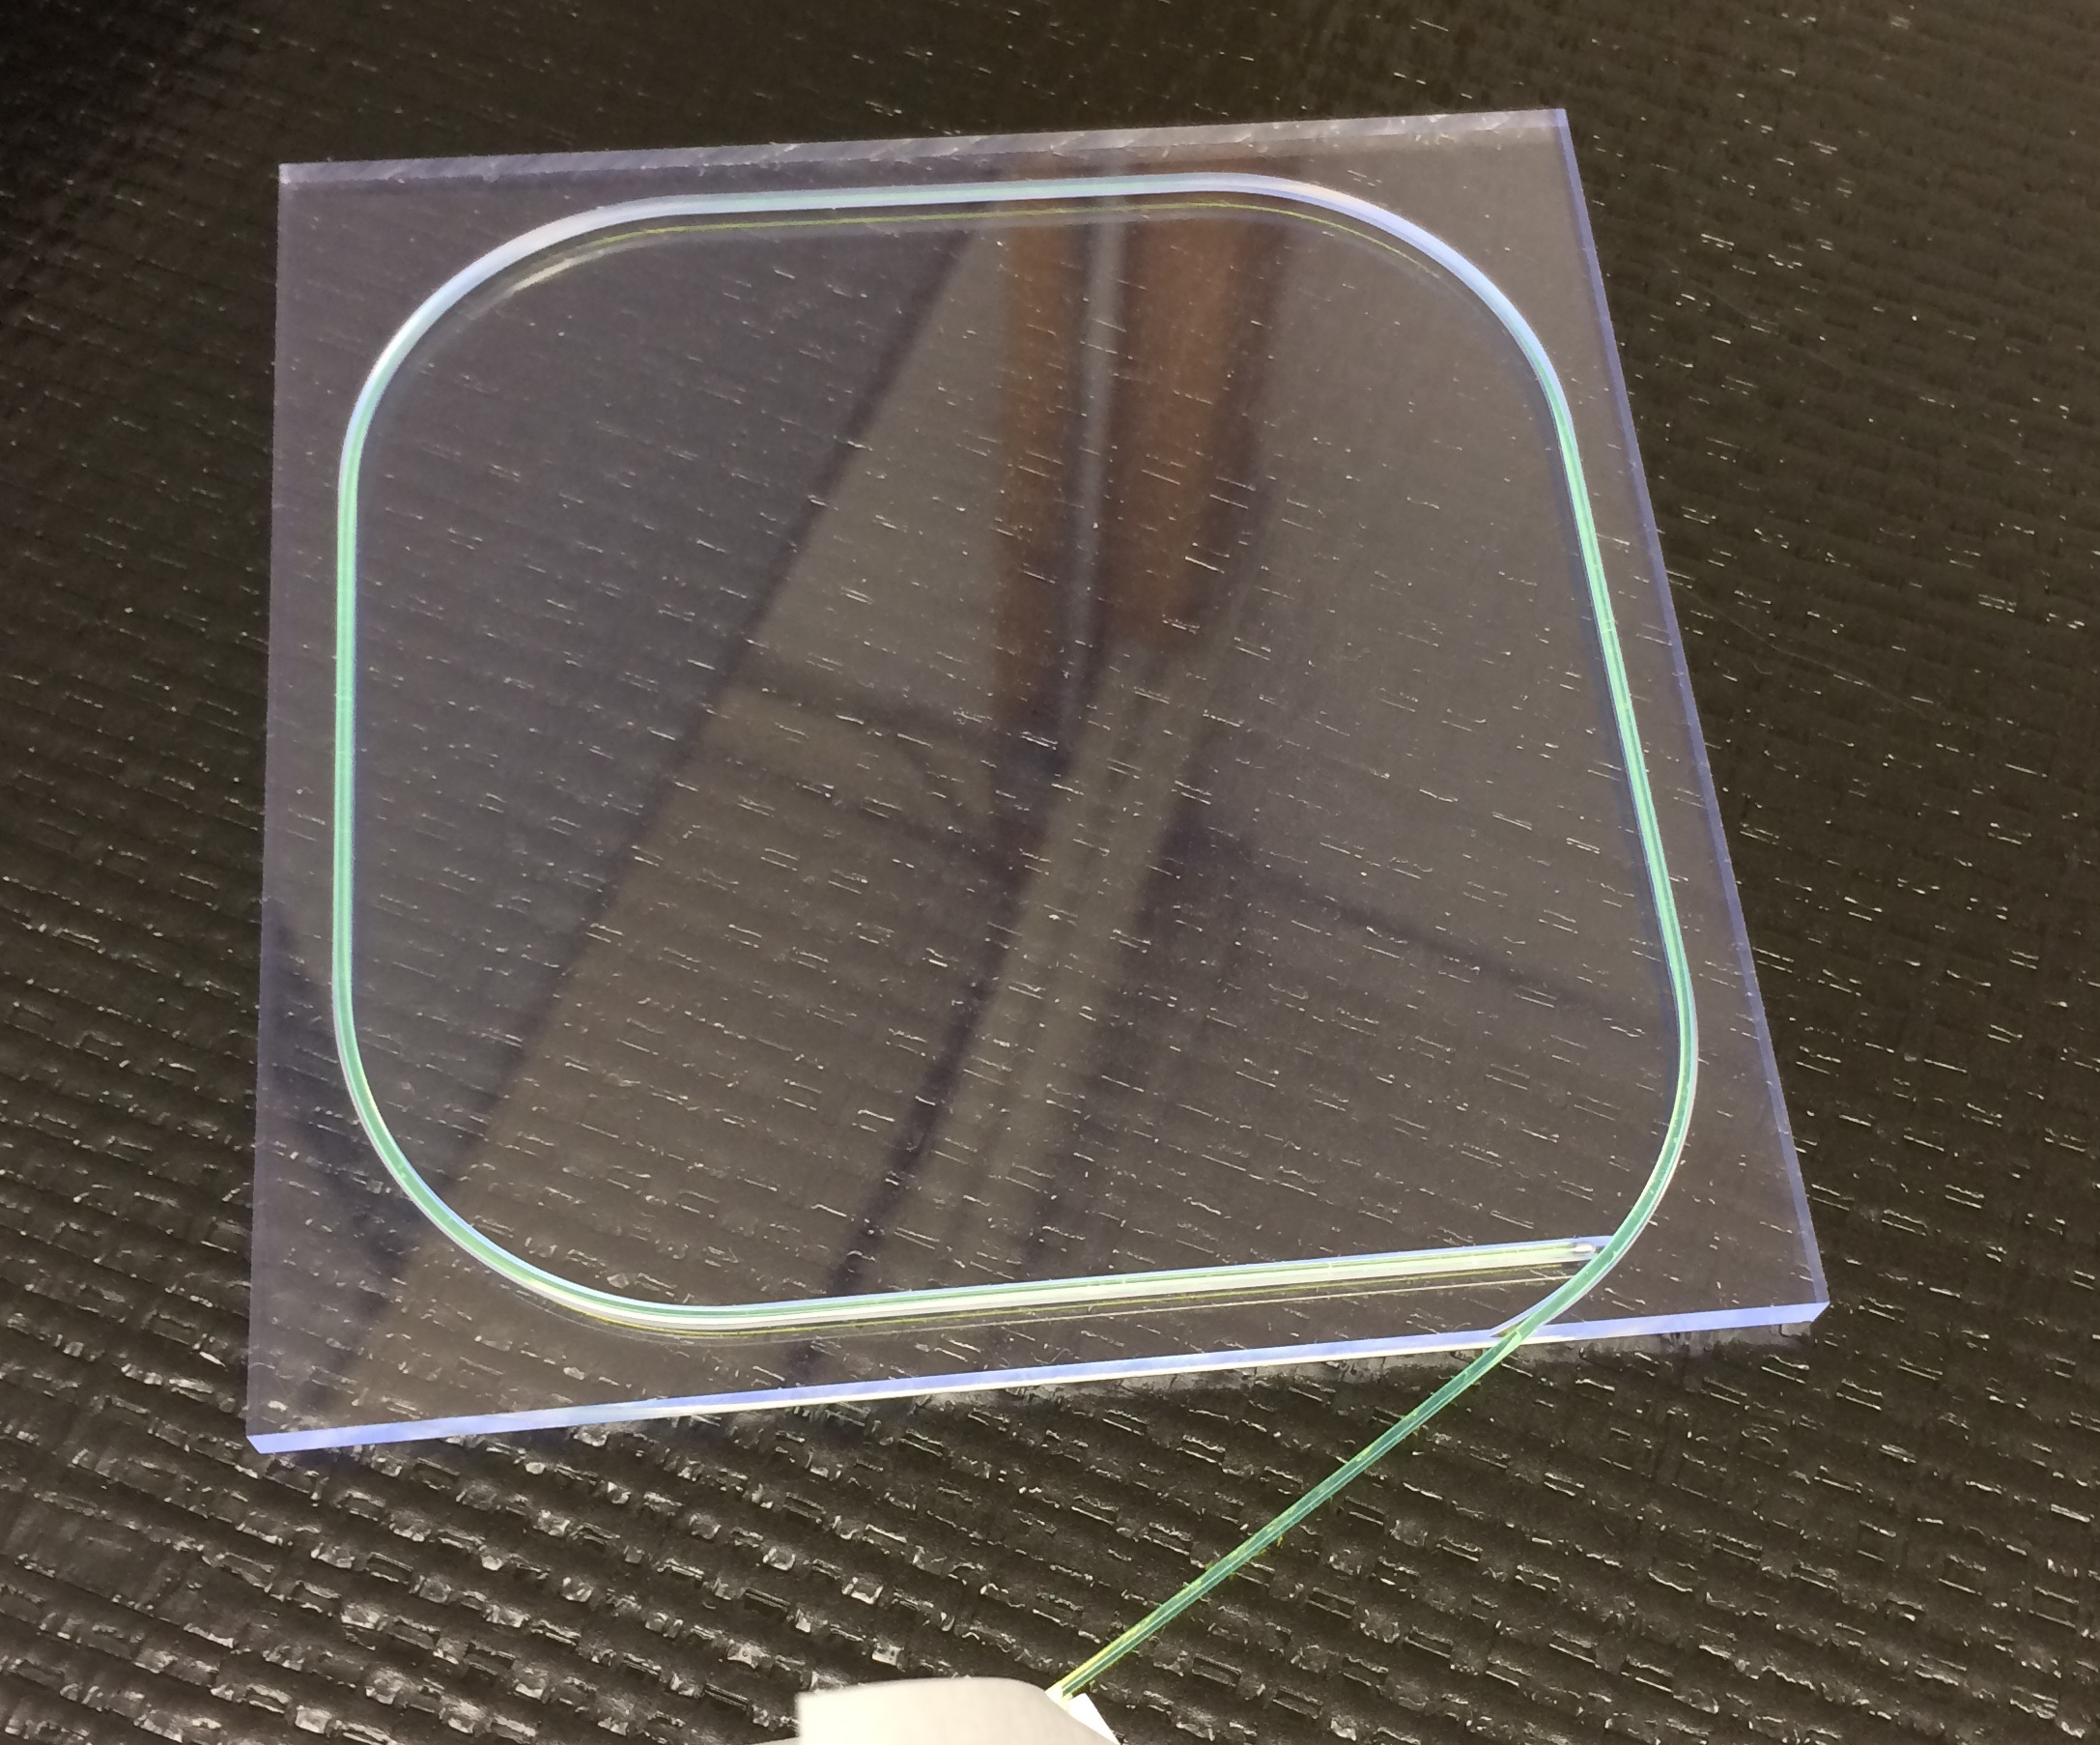
\includegraphics[width=0.4\textwidth]{figures/sigma}
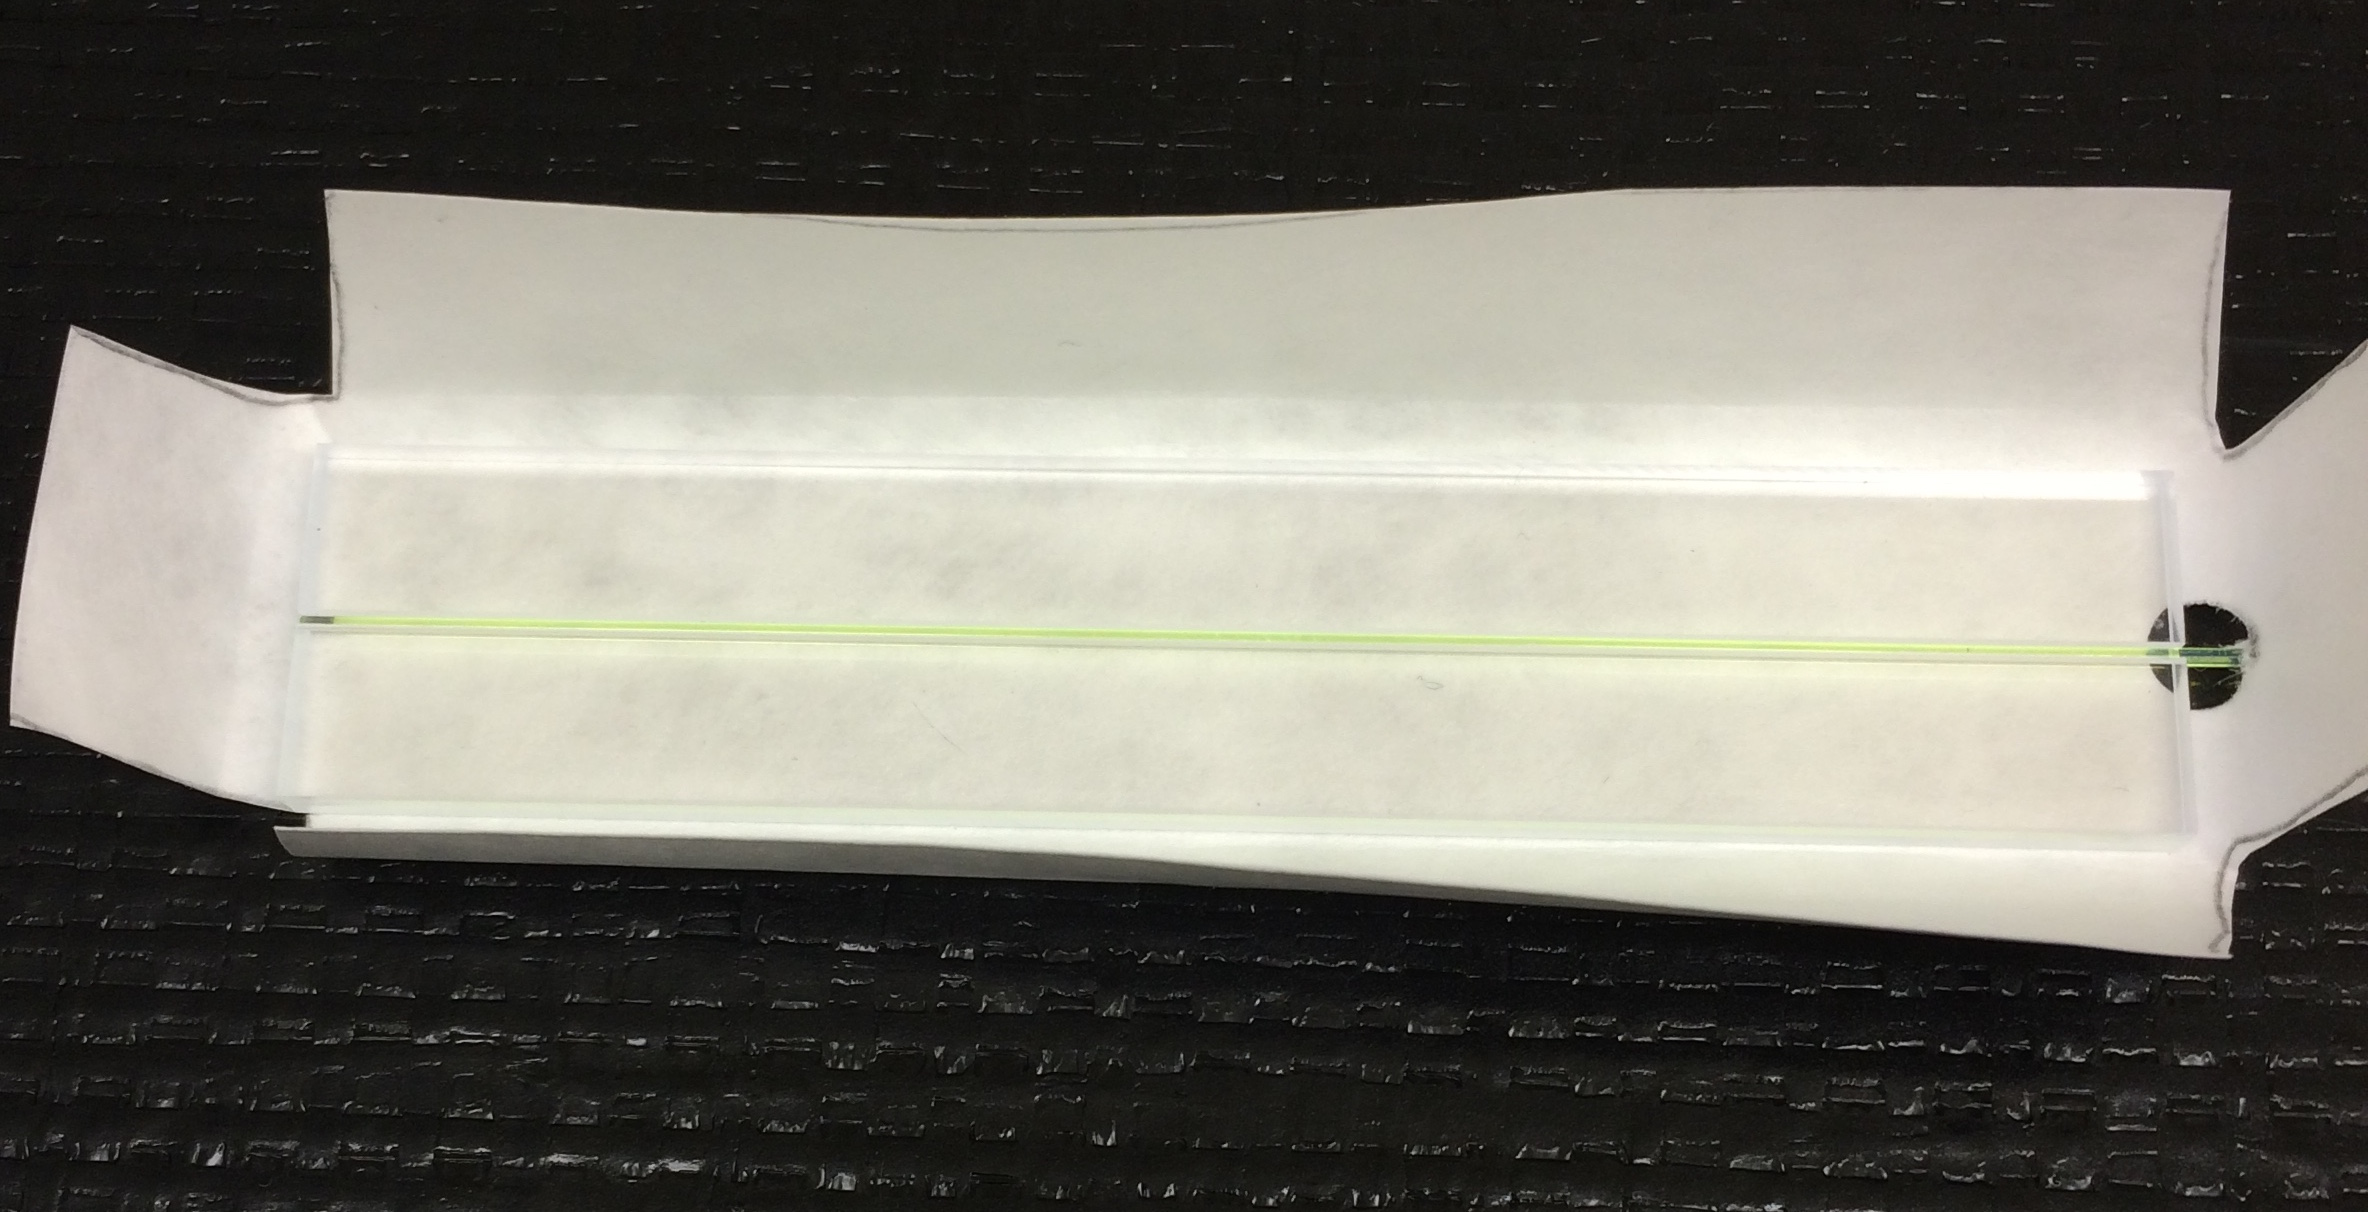
\includegraphics[width=0.4\textwidth]{figures/finger-horizontal}
\caption{(\cmsLeft) Sigma tile with green WLS fiber. (\cmsRight) Finger tile with green WLS fiber, lying on Tyvek wrapping.}
\label{fig:sigma-finger}
\end{center}
\end{figure}

In this experiment, there are two tiles with special geometries.
\begin{itemize}
\item \textbf{Multi-pronged sigma tile:} Two of the sigma tiles, instead of having a single WLS fiber with a sigma-shaped trajectory, have instead a number of straight, parallel WLS fibers running through them. Laser light is shined onto the tile above the center of each of the straight WLS fibers, as though they were finger tile WLS fibers. The signals from the fibers are read out separately by the readout system. One of these special tiles has four WLS fibers, with laser light fibers shining onto each of them. The other tile has three WLS fibers, two of which have a laser light fiber shining onto them, while the third does not and only receives scintillation light produced in the tile by the other two laser fibers that do not shine directly onto it. These two special sigma tile geometries will be referred to respectively as 4-pronged sigma tile and 3-pronged sigma tile.
\item \textbf{Truncated finger tile:} One of the finger tiles is only 5 cm long instead of 10 cm; all the other dimensions are normal.
\end{itemize}

The scintillator materials used in this study are:

\begin{table}[htbh]
\begin{center}
\topcaption{Properties of the scintillator materials analyzed for radiation tolerance on the CASTOR table: photons per 1-MeV electron, peak wavelength of emission, decay time, and base material. Some properties are not listed for Scintillator X because the material has not been patented yet. Guide to base material acronyms: PS = polystyrene. PVT = polyvinyltoluene. \label{tab:scint-materials}}
\begin{tabular}{|c|c|c|c|c|}
\hline
Material & $\gamma$/1MeV-$e$ yield & $\lambda_{em}$ (nm) & Decay time (ns) & Base material \\
\hline
\hline
SCSN81~\cite{Kuraray} &  & 430 & 2.5 & PS \\
EJ200~\cite{EJ200} & 10000 & 425 & 2.1 & PVT \\
EJ260~\cite{EJ260} & 9200 & 490 & 9.2 & PVT \\
Scintillator X &  &  &  &  \\
LS6946 &  &  &  & Polysiloxane \\
PTP &  &  &  &  \\
PEN &  &  &  &  \\
PET &  &  &  &  \\
\hline
\end{tabular}
\end{center}
\end{table}

\begin{table}[htbh]
\begin{center}
\topcaption{Properties of the wavelength-shifters (WLS) used in this experiment: material type, the tiles they were used with, peak wavelength of absorption, peak wavelength of emission, and diameter. The second column lists the types of scintillator material (see Table~\ref{tab:scint-materials}) that each WLS was used with. All WLS fibers were multi-cladded, with numerical aperture 0.72, trapping efficiency 5.4\%, and cladding thickness equal to 4\% of their diameter~\cite{KuraWLS}.\label{tab:WLS-materials}}
\begin{tabular}{|c|c|c|c|c|}
\hline
Material & Used with tile(s) & $\lambda_{abs}$ (nm) & $\lambda_{em}$ (nm) & Diameter (mm) \\
\hline
Y11~\cite{KuraWLS} & SCSN81, EJ200, Scint. X, PEN & 430 & 476 & 0.94 \\
O2~\cite{KuraWLS} & EJ260 & 535 & 550 & 0.98 \\
B2~\cite{KuraWLS} & PTP, PET & 375 & 437 & 0.98 \\
\hline
\end{tabular}
\end{center}
\end{table}

The scintillator samples are wrapped individually in reflective Tyvek material and stored inside black plastic cassettes to isolate them from external light. One cassette can hold either one sigma tile or up to four finger tiles. Figures~\ref{fig:sigmatile}-~\ref{fig:fingertile} show how wrapped sigma tiles and finger tiles are arranged inside their cassettes. There are a few tiles with exceptional shapes: Scintillator X (Figure~\ref{fig:scintXtile}) has a truncated finger geometry, and PTP (Figure~\ref{fig:PTPtile}) and PEN (Figure~\ref{fig:PENtile}) have 4-pronged and 3-pronged sigma tile geometries respectively; the third WLS fiber in the PEN tile does not have a laser fiber shining onto it.

\begin{figure}[hbtp]
\begin{center}
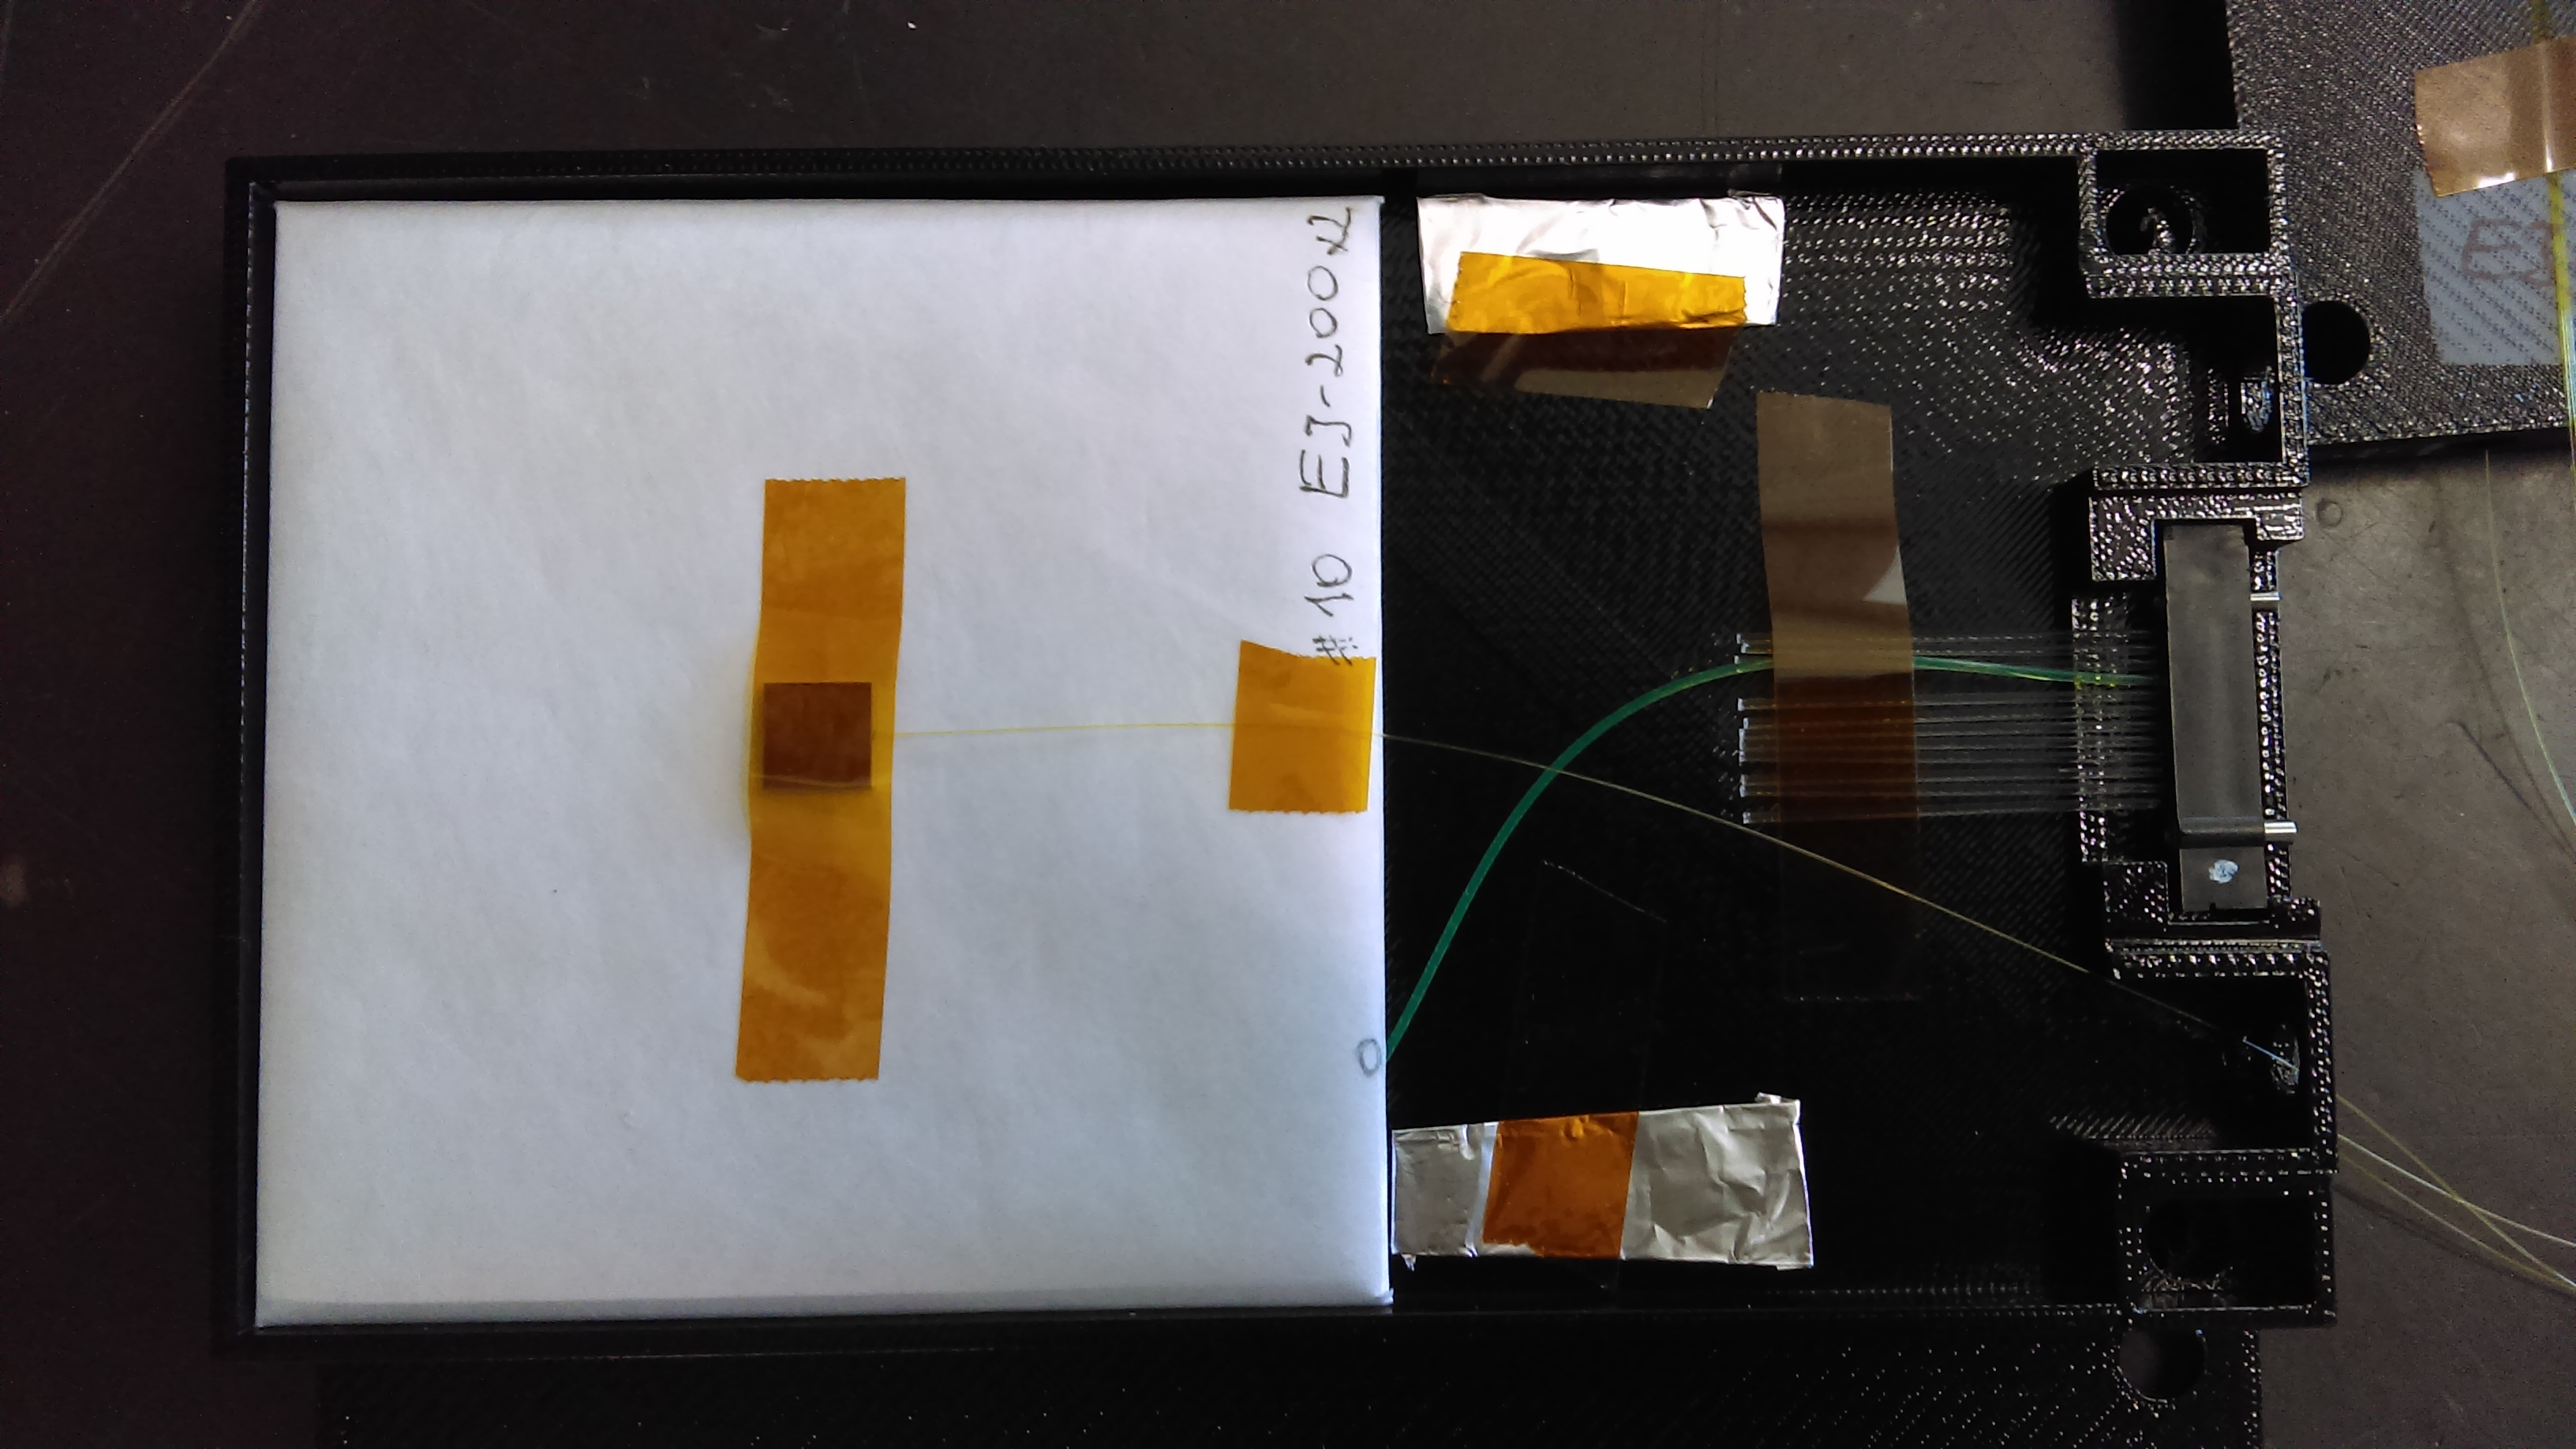
\includegraphics[width=0.75\textwidth]{figures/sigmatile}
\caption{EJ200 sigma tile inside a cassette.}
\label{fig:sigmatile}
\end{center}
\end{figure}

\begin{figure}[hbtp]
\begin{center}
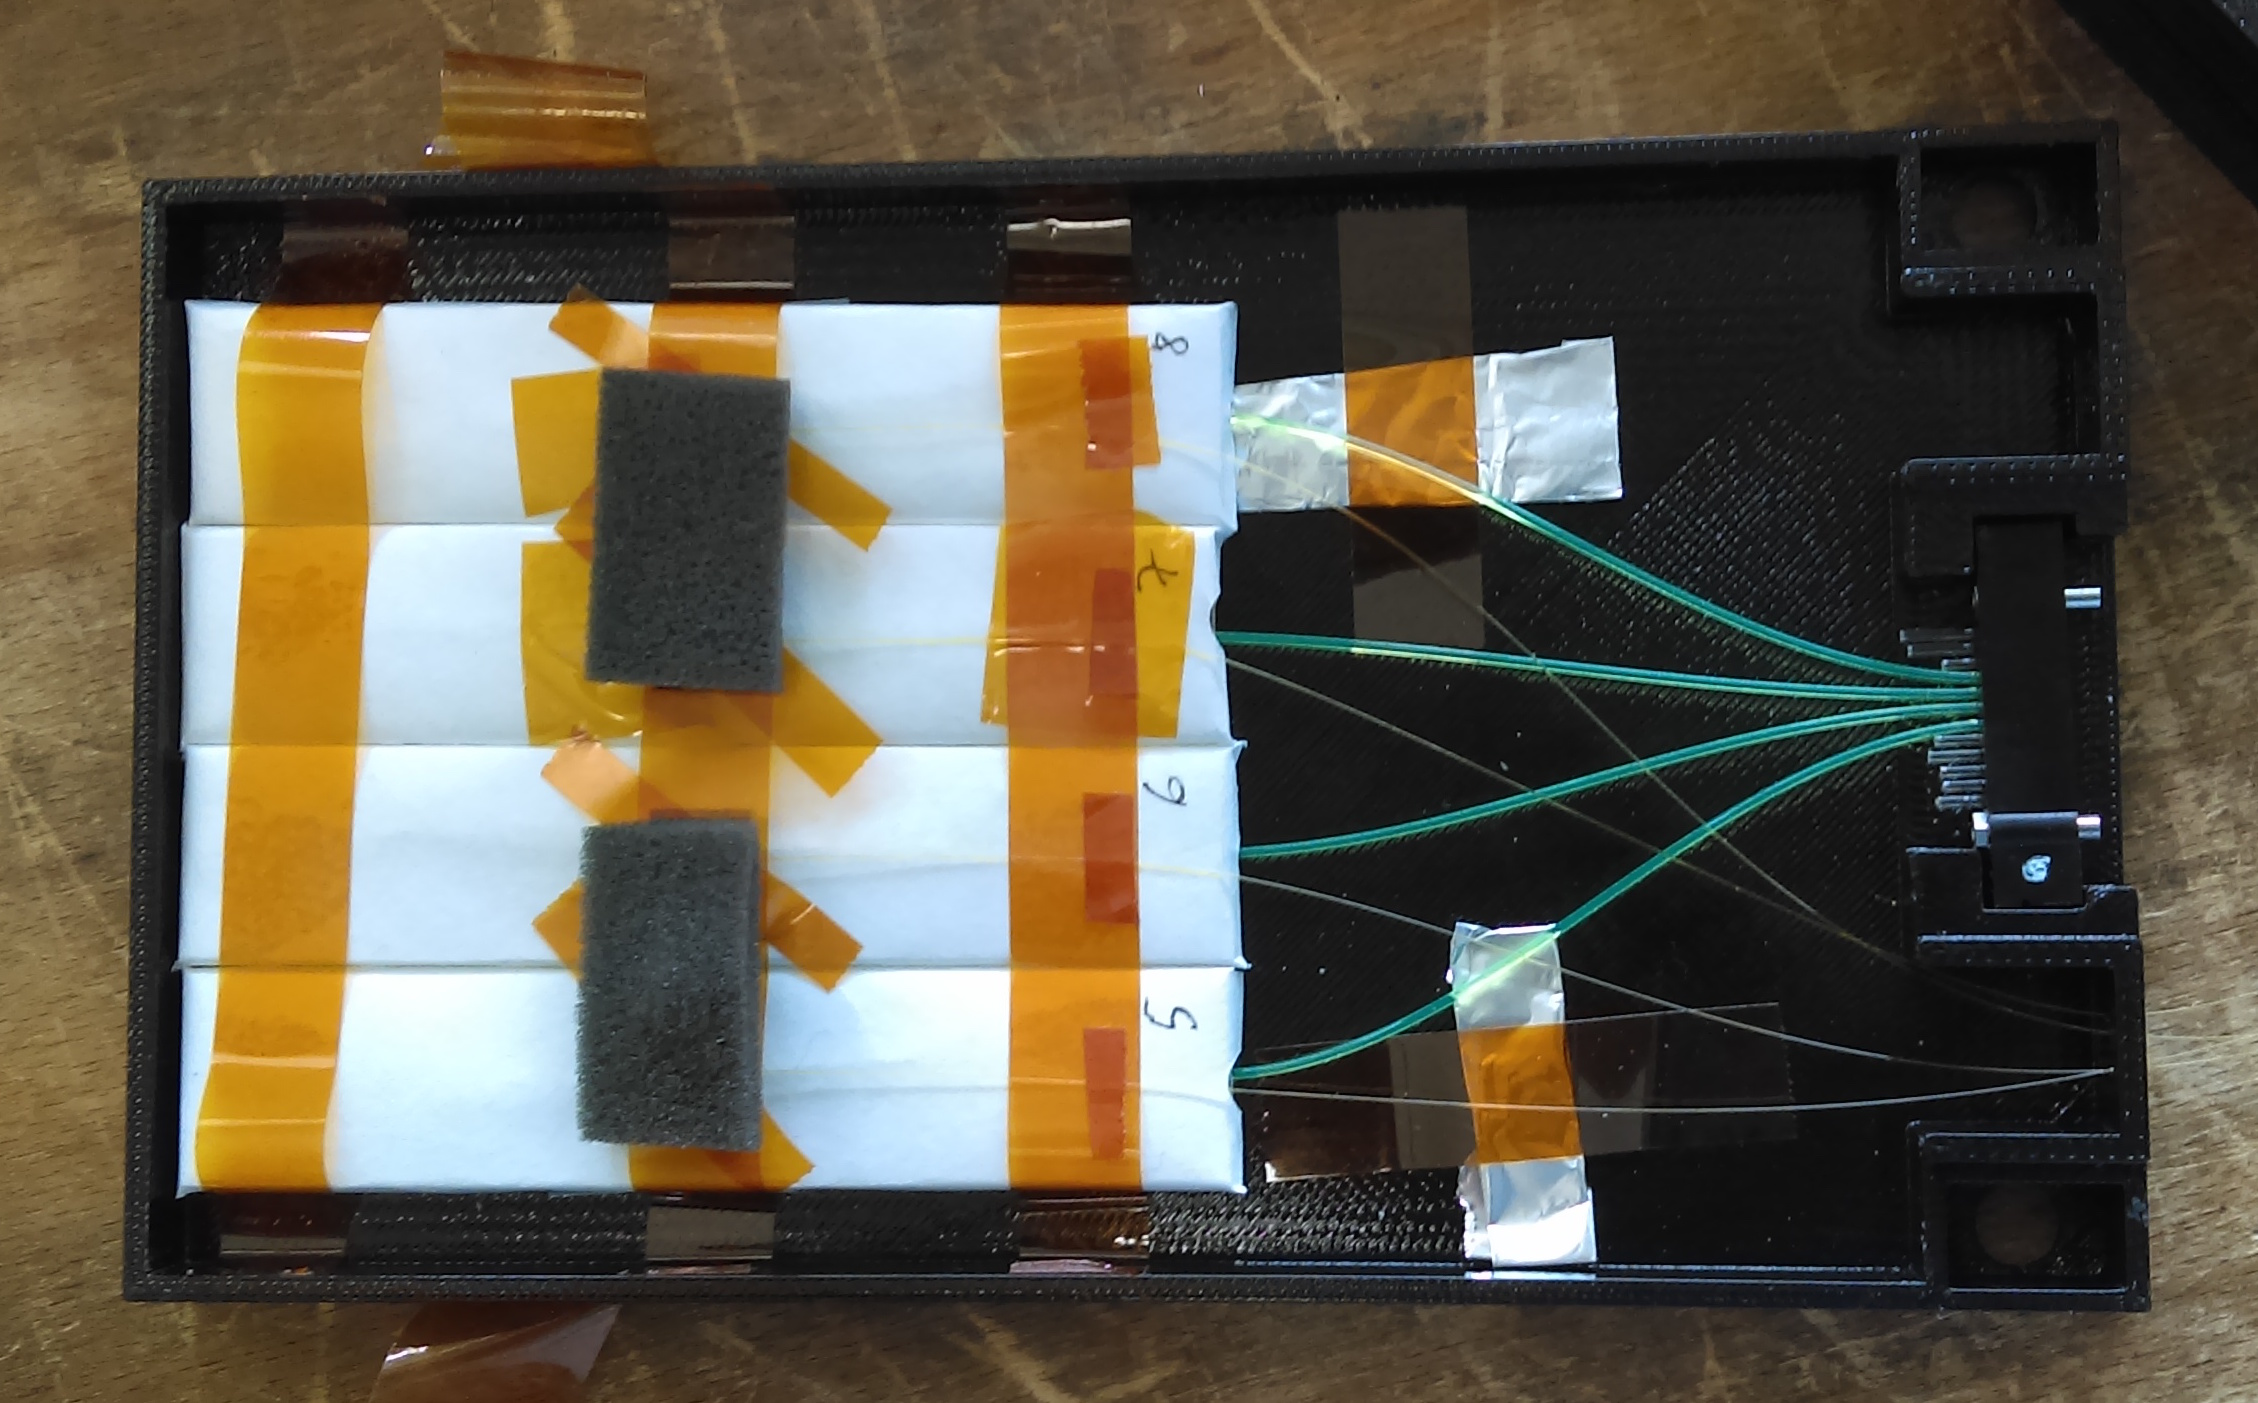
\includegraphics[width=0.75\textwidth]{figures/fingertile}
\caption{SCSN-81 finger tiles inside a cassette.}
\label{fig:fingertile}
\end{center}
\end{figure}

\begin{figure}[hbtp]
\begin{center}
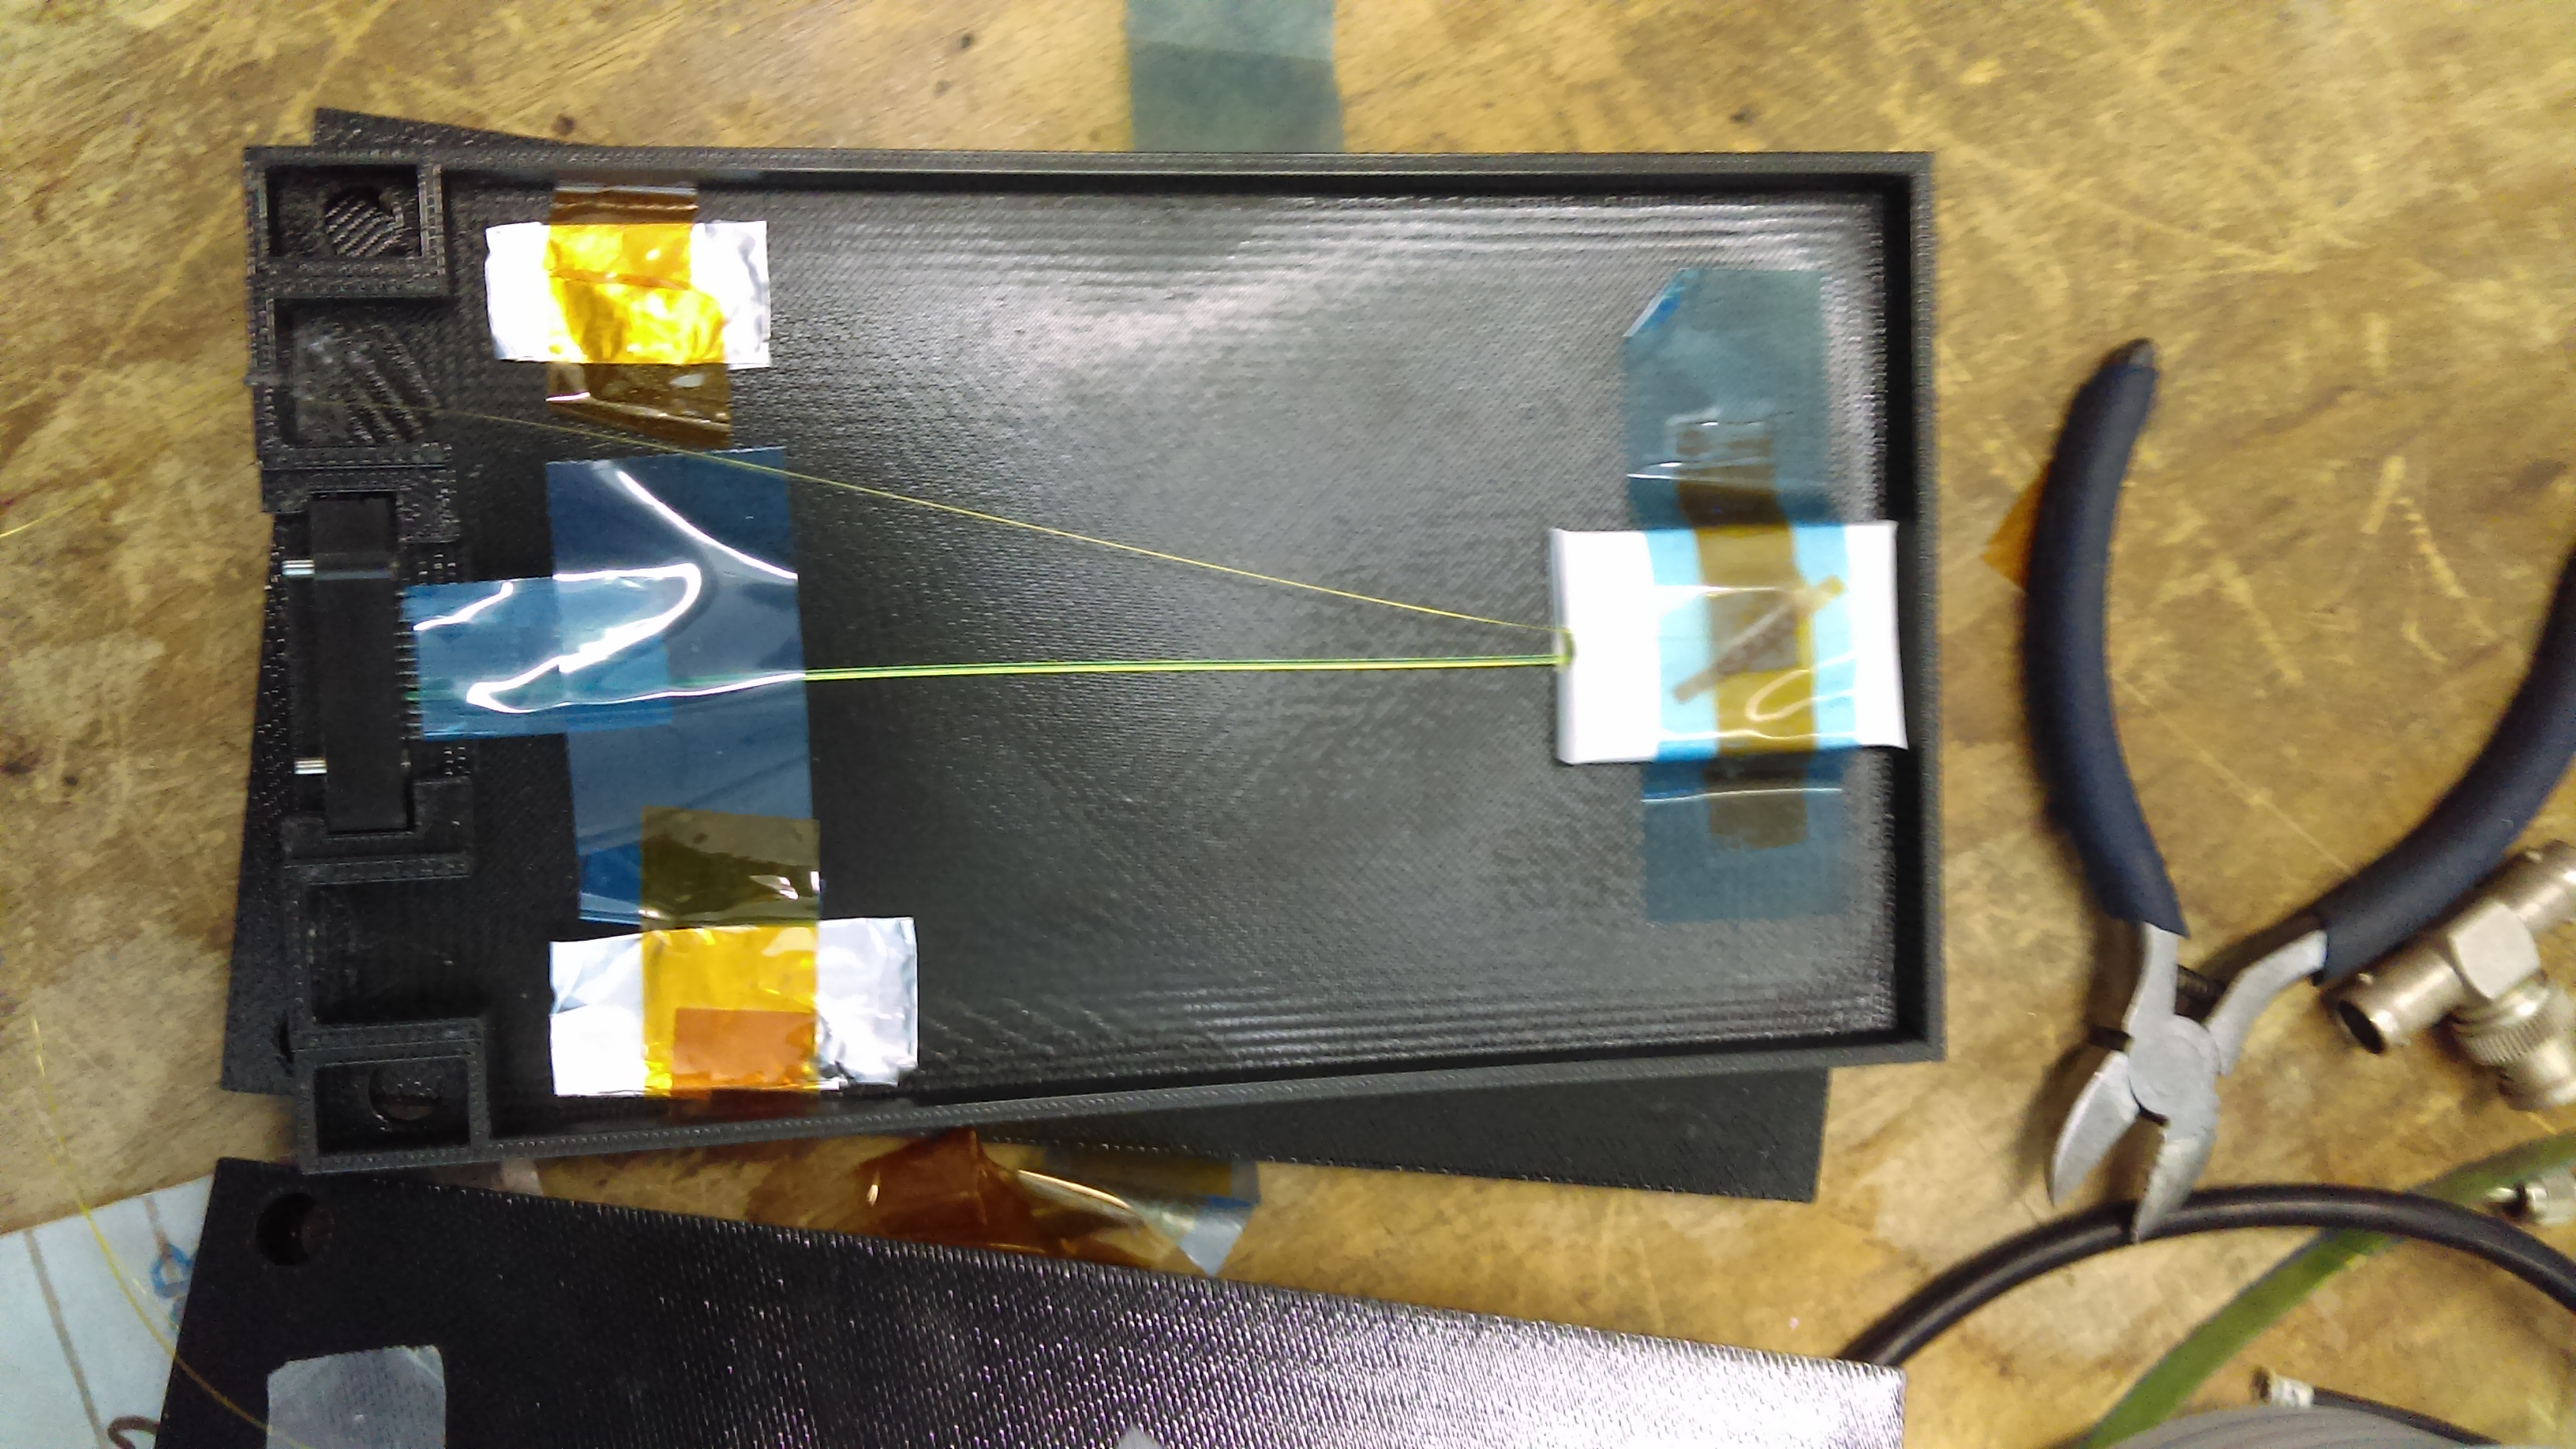
\includegraphics[width=0.75\textwidth]{figures/scintXtile}
\caption{Scintillator X truncated finger tile inside a cassette.}
\label{fig:scintXtile}
\end{center}
\end{figure}

\begin{figure}[hbtp]
\begin{center}
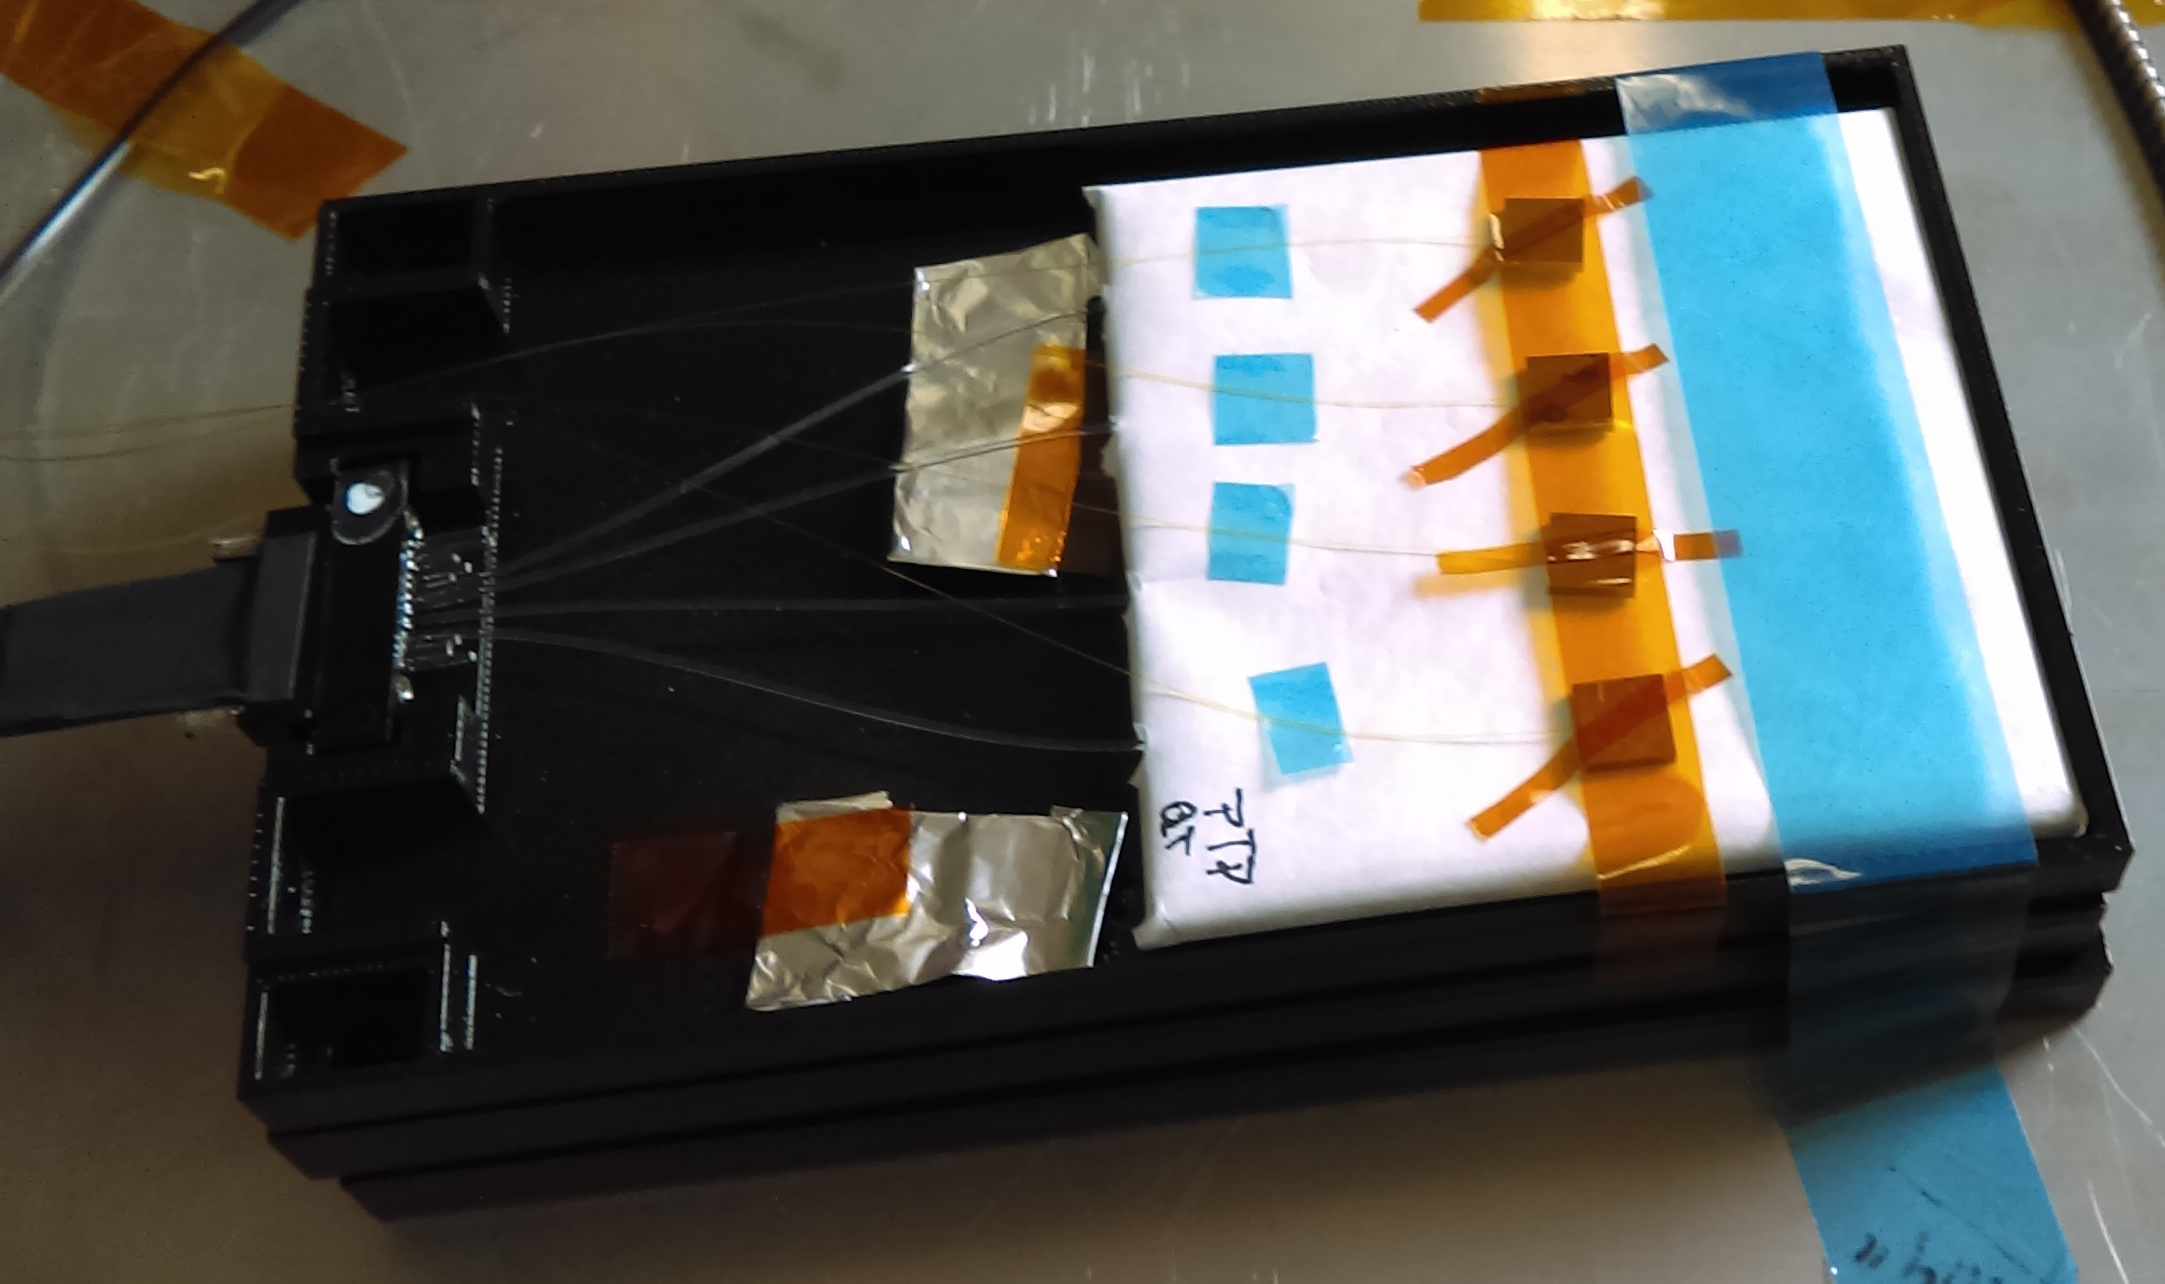
\includegraphics[width=0.75\textwidth]{figures/PTPtile}
\caption{PTP 4-pronged sigma tile inside a cassette.}
\label{fig:PTPtile}
\end{center}
\end{figure}

\begin{figure}[hbtp]
\begin{center}
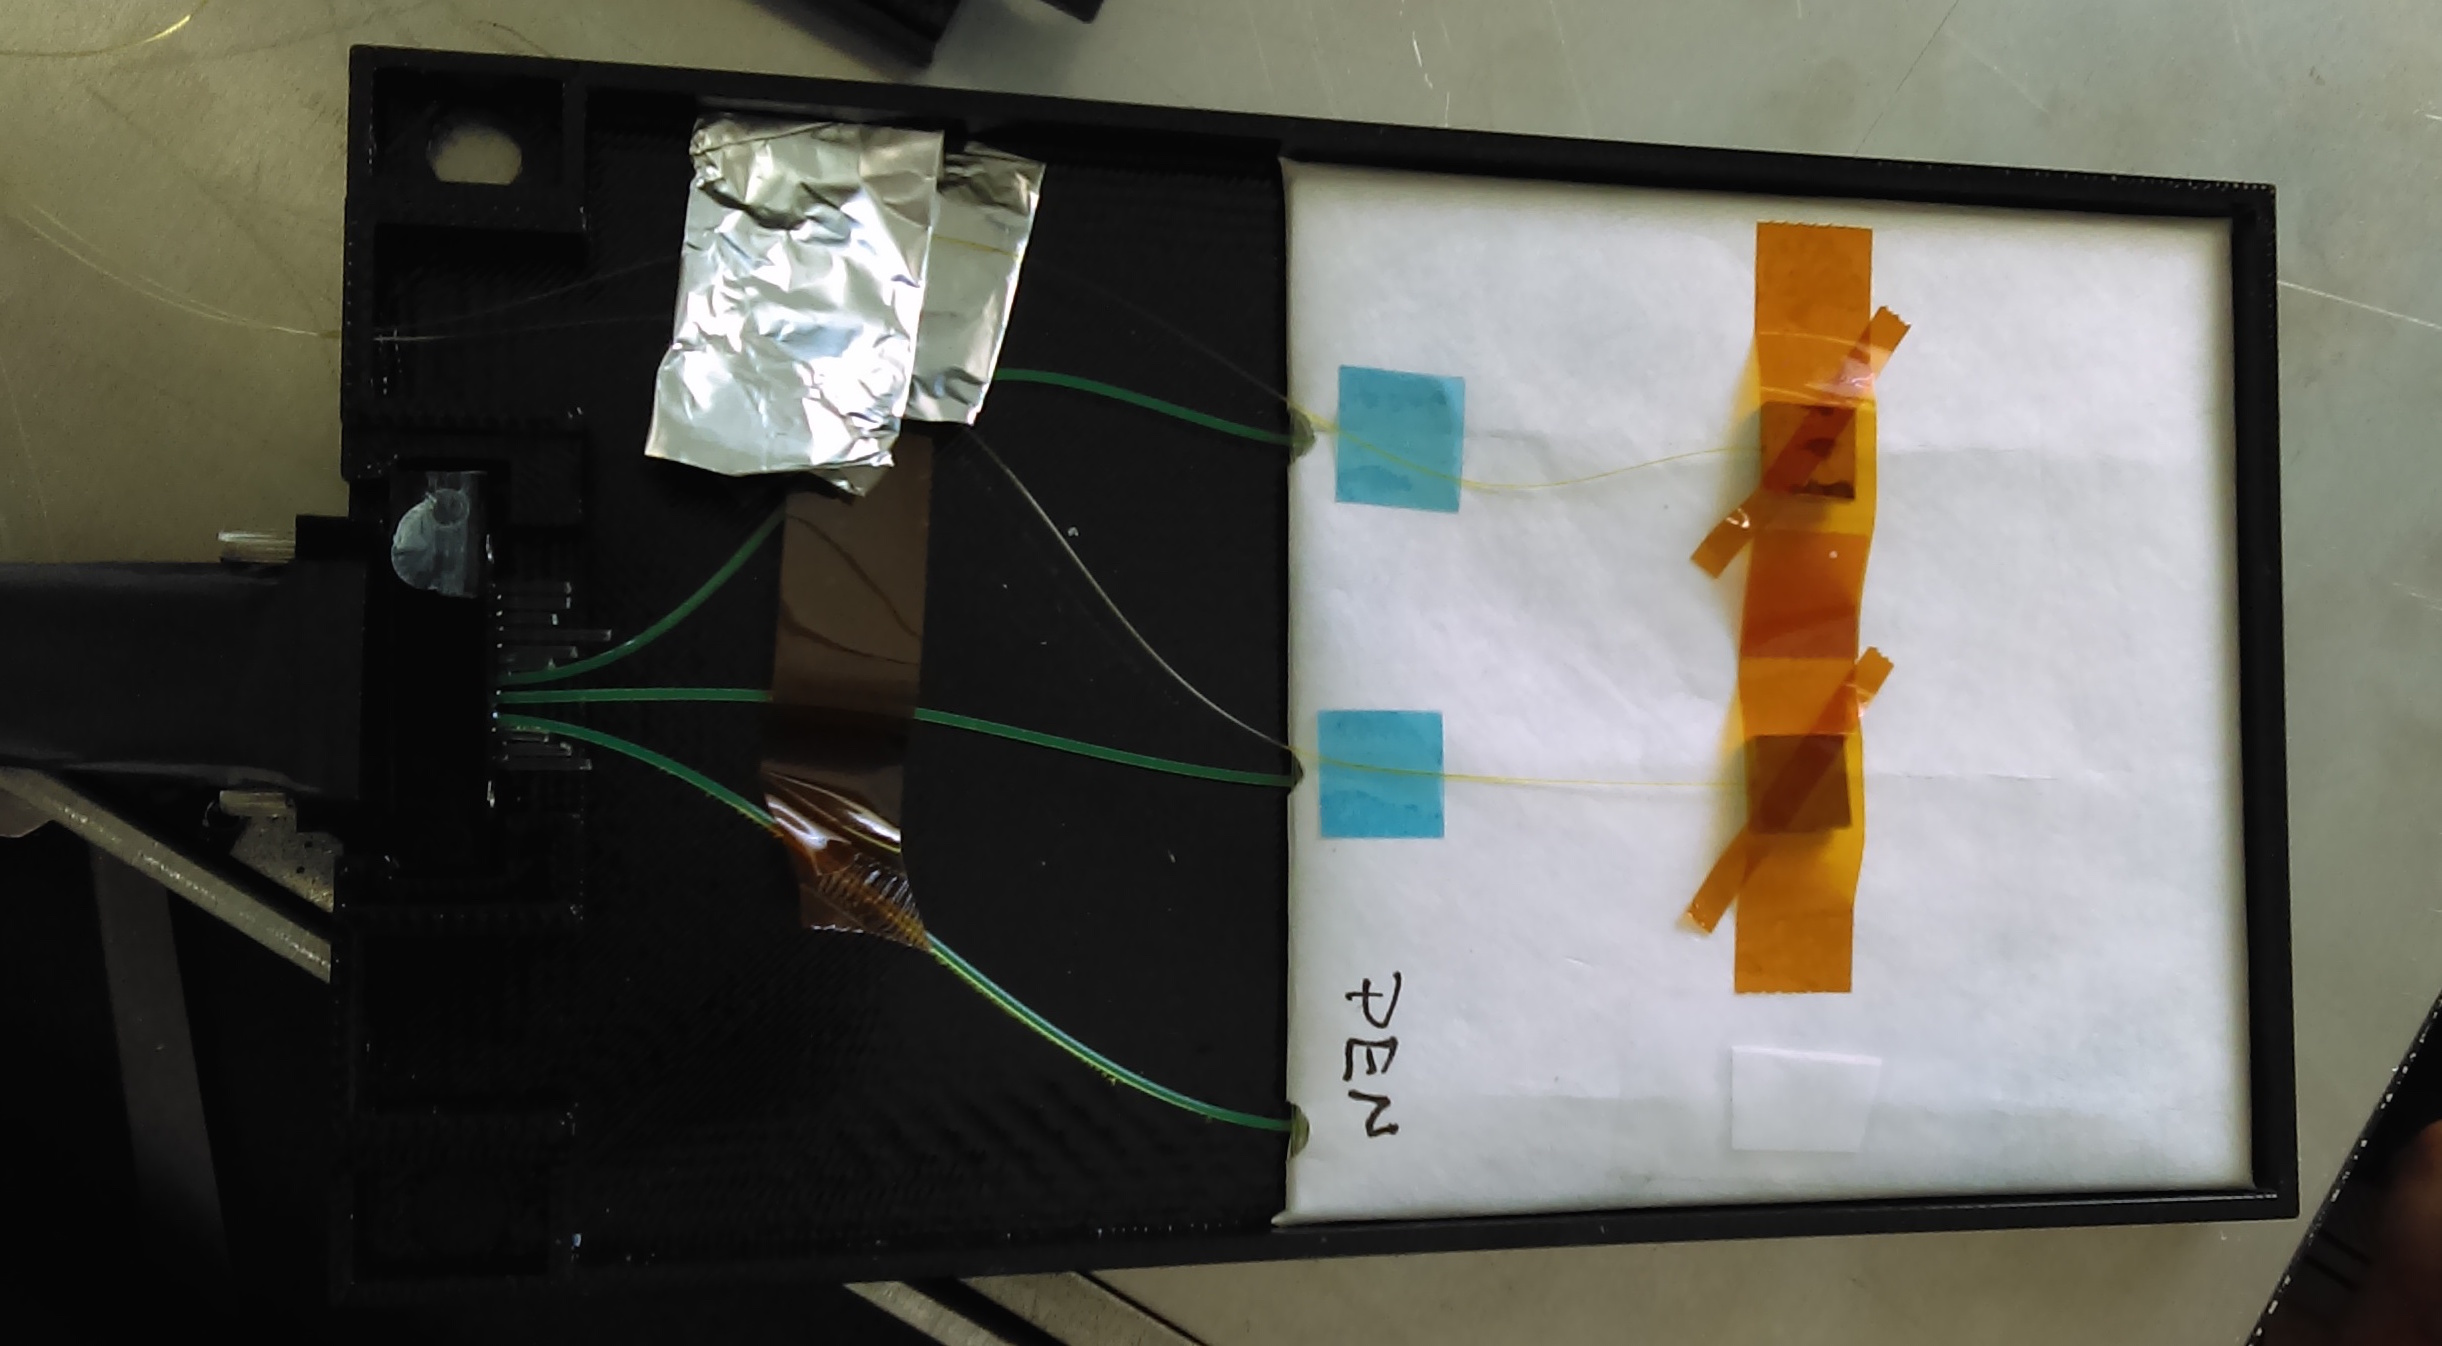
\includegraphics[width=0.75\textwidth]{figures/PENtile}
\caption{PEN 3-pronged sigma tile inside a cassette. One of the WLS fibers was intentionally left without a laser fiber illuminating it.}
\label{fig:PENtile}
\end{center}
\end{figure}

\subsection{Dark Boxes\label{sec:setup-darkboxes}}

The scintillator samples inside their cassettes are to be placed on the CRF platform to be irradiated close the LHC beam-pipe, at an expected dose rate of $\mathcal{O}$(1-10) krad/hr, depending on the distance from the beampipe. Two ``Dark Boxes" with dimensions 39.9 cm $\times$ 34.8 cm $\times$ 18.1 cm have been designed and built by Fermilab to hold the cassettes. Each box can hold 24 cassettes and also contains a laser light injection box that splits uniformly the incoming laser light among the cassettes, a system of plastic tubes for circulating dry air through the cassettes to keep the environmental humidity low, and a system of clear fibers that carry scintillation light from individual tiles.

Light of wavelength 351 nm from the USC laser source at Point 5 is used to illuminate the scintillators. The laser light reaching the light injection box is split between nine identical outputs. To each of these outputs is connected a bundle of CeramOptec quartz core-fibers with core cladding (core diameter 250 $\mu$m and total diameter 280 $\mu$m including cladding). From these bundles, one or more laser fibers enter each cassette to illuminate the scintillator sample(s) within. Inside the cassette, each laser fiber terminates at a metallic mirror that directs the light onto a dedicated scintillator sample through a hole in the Tyvek covering; the hole is small enough that the metallic mirror, lying directly on top of it, blocks any other light from entering except the light from the laser fiber. The scintillation light produced in each tile is collected by a WLS fiber (see Table~\ref{tab:WLS-materials} for the materials and dimensions of the various WLS fibers used) which is spliced to a 0.94 mm-diameter, multi-cladded clear fiber~\cite{KuraWLS} as it exits the cassette.

Inside the Dark Box, the cassettes are arranged in stacks of 6 or 9. When the Dark Box is placed under the beam pipe, the cassette stacks are all located directly below the beampipe at the same azimuthal ($\phi$) position, and thus the distances of the various tiles from the beam axis differ only in the radial dimension r. Tables~\ref{tab:distances-box1} and~\ref{tab:distances-box2} list the distances, in Dark Boxes 1 and 2 respectively, of each scintillator material sample from the beampipe.

\begin{table}
\begin{center}
\begin{tabular}{|c|c|c|}
\hline
Material & Shapes & Distance (cm) \\
\hline
\multirow{9}{*}{SCSN81} & 1S & 11.8 \\
& 1S & 13.1 \\
& 4F & 14.4 \\
& 1S & 18.2 \\
& 1S & 19.5 \\
& 4F & 20.8 \\
& 2S & 24.6 \\
& 2S & 25.9 \\
& 6F & 27.2 \\
\hline
\multirow{2}{*}{EJ200} & 1S & 13.1 \\
& 1S & 19.5 \\
\hline
\multirow{7}{*}{EJ260} & 2S & 11.8 \\
& 1S & 13.1 \\
& 4F & 14.4 \\
& 1S & 18.2 \\
& 2F & 20.8 \\
& 1S & 24.6 \\
& 2F & 27.2 \\
\hline
\end{tabular}
\caption{Table of scintillator samples in Dark Box 1 and their respective distances from the beamline in cm. The first column lists the material type. The second column lists the number of tiles with sigma (S) and finger (F) shapes; for example, an entry of "4F" means that there are four finger tiles at this radius from the beamline. The third column lists the distance from the beamline. The uncertainty of the distance measurements is conservatively estimated to be +/-1 cm.}
\label{tab:distances-box1}
\end{center}
\end{table}

\begin{table}
\begin{center}
\begin{tabular}{|c|c|c|}
\hline
Material & Shapes & Distance (cm) \\
\hline
\multirow{9}{*}{SCSN81} & 1S & 11.8 \\
& 1S & 13.1 \\
& 4F & 14.4 \\
& 2S & 18.2 \\
& 2S & 19.5 \\
& 4F & 20.8 \\
& 3S & 24.6 \\
& 2S & 25.9 \\
& 4F & 27.2 \\
\hline
\multirow{4}{*}{EJ200} & 1S & 11.8 \\
& 1S & 13.1 \\
& 1S & 19.5 \\
& 1S & 25.9 \\
\hline
PTP & 1S(4-prong) & 11.8 \\
\hline
PEN & 1S(3-prong) & 13.1 \\
\hline
PET & 1S & 14.4 \\
\hline
Scintillator X & 1F(truncated) & 13.1 \\
\hline
LS6946 & 2F & 27.2 \\
\hline
\end{tabular}
\caption{Table of scintillator samples in Dark Box 2 and their respective distances from the beamline in cm. The first column lists the material type. The second column lists the number of tiles with sigma (S) and finger (F) shapes; for example, an entry of "4F" means that there are four finger tiles at this radius from the beamline. The third column lists the distance from the beamline. The uncertainty of the distance measurements is conservatively estimated to be +/-1 cm. N.B.: scintillator X, PTP, and PEN all have special tile geometries, described in Sec.~\ref{sec:setup-tiles}.}
\label{tab:distances-box2}
\end{center}
\end{table}

Figure~\ref{fig:box-schematic} shows the arrangement of the cassette stacks inside Dark Boxes 1 and 2; the material of each scintillator sample is indicated, as well as its shape (``S" at the end of the name stands for sigma tile, and ``F" stands for finger tile). Figures~\ref{fig:dark-box-1} and~\ref{fig:dark-box-2} show exterior and interior views respectively of a Dark Box.

\begin{figure}[hbtp]
\begin{center}
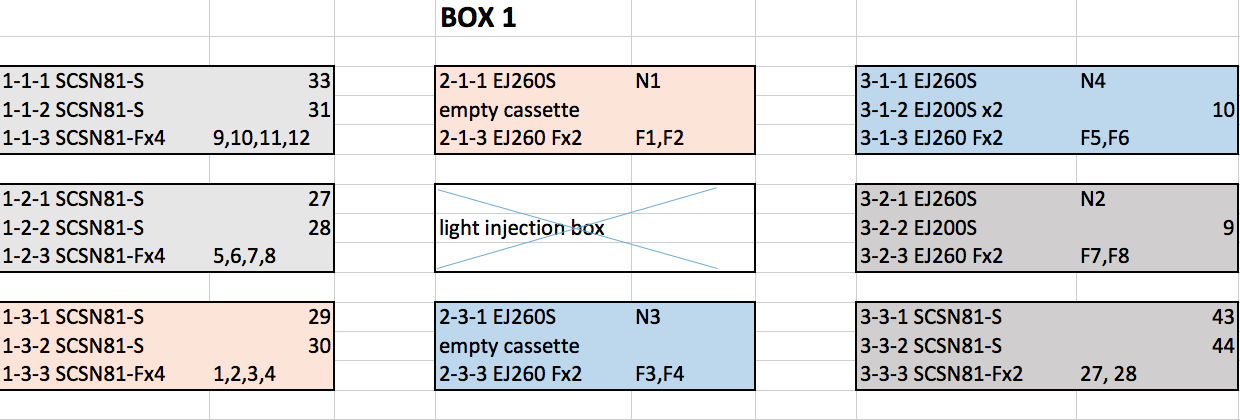
\includegraphics[width=0.8\textwidth]{figures/Box1_SamplesMap}
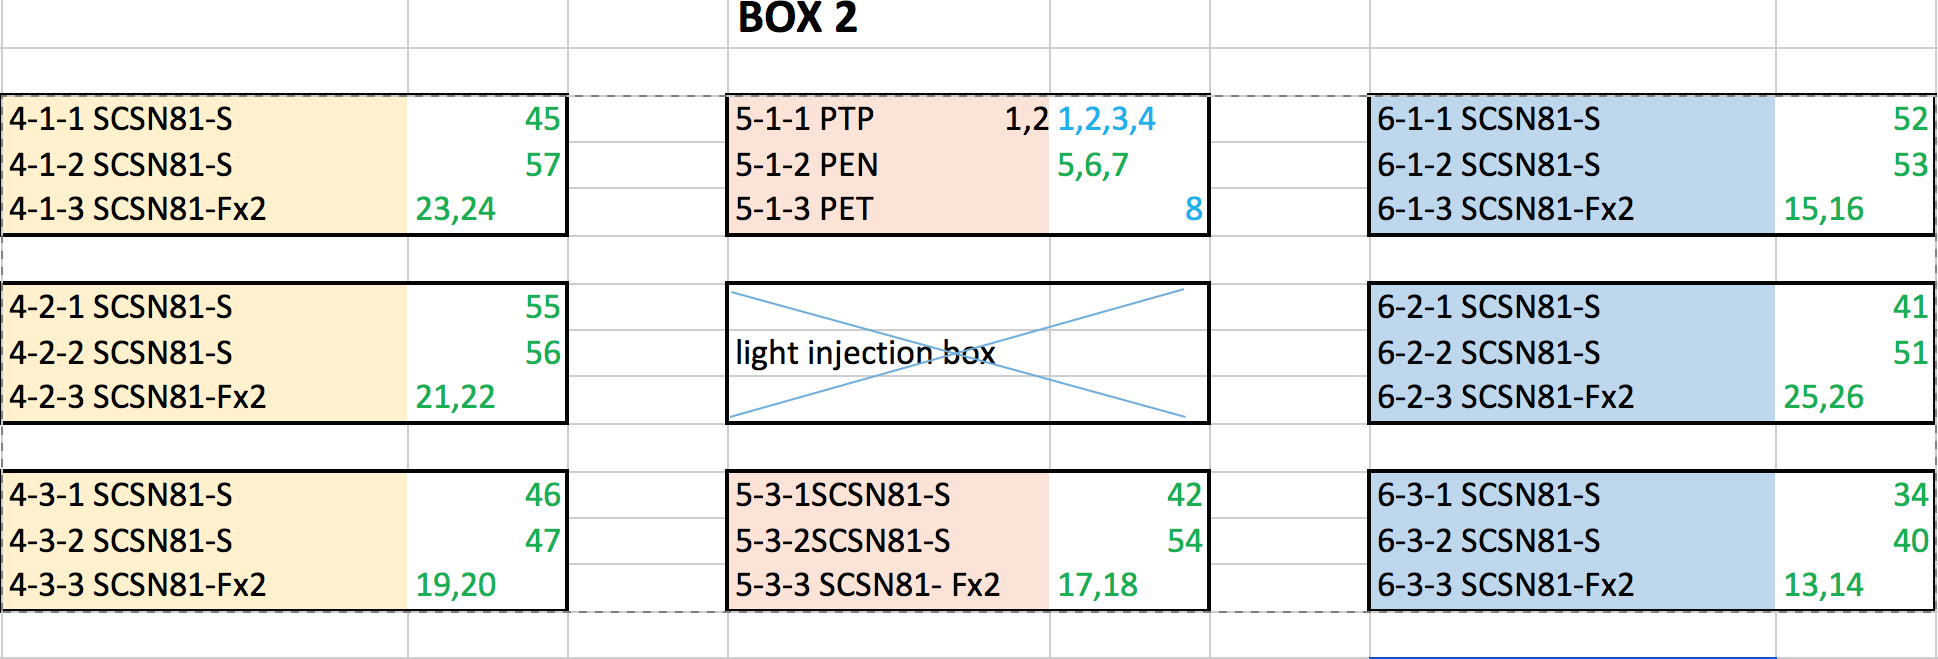
\includegraphics[width=0.8\textwidth]{figures/Box2_SamplesMap}
\caption{(Top) Arrangement of cassettes inside Dark Box 1. (Bottom) Arrangement of cassettes inside Dark Box 2. In these diagrams, the numbered labels ``X-Y-Z" on the left-hand side of each stack identify the cassette positions inside the box. The numbers at the right-hand side of each stack are used to connect the cassettes correctly to the clear fibers that carry the scintillation light out of the Dark Box. When the Dark Boxes are on the CASTOR table, the beam pipe (z-axis) runs from left to right across the top of each figure, meaning that cassettes numbered ``X-1-1" are closest to the beampipe and that those numbered ``X-3-3" are farthest from the beampipe. All cassettes in the same row are at the same distance from the beampipe.}
\label{fig:box-schematic}
\end{center}
\end{figure}

\begin{figure}[hbtp]
\begin{center}
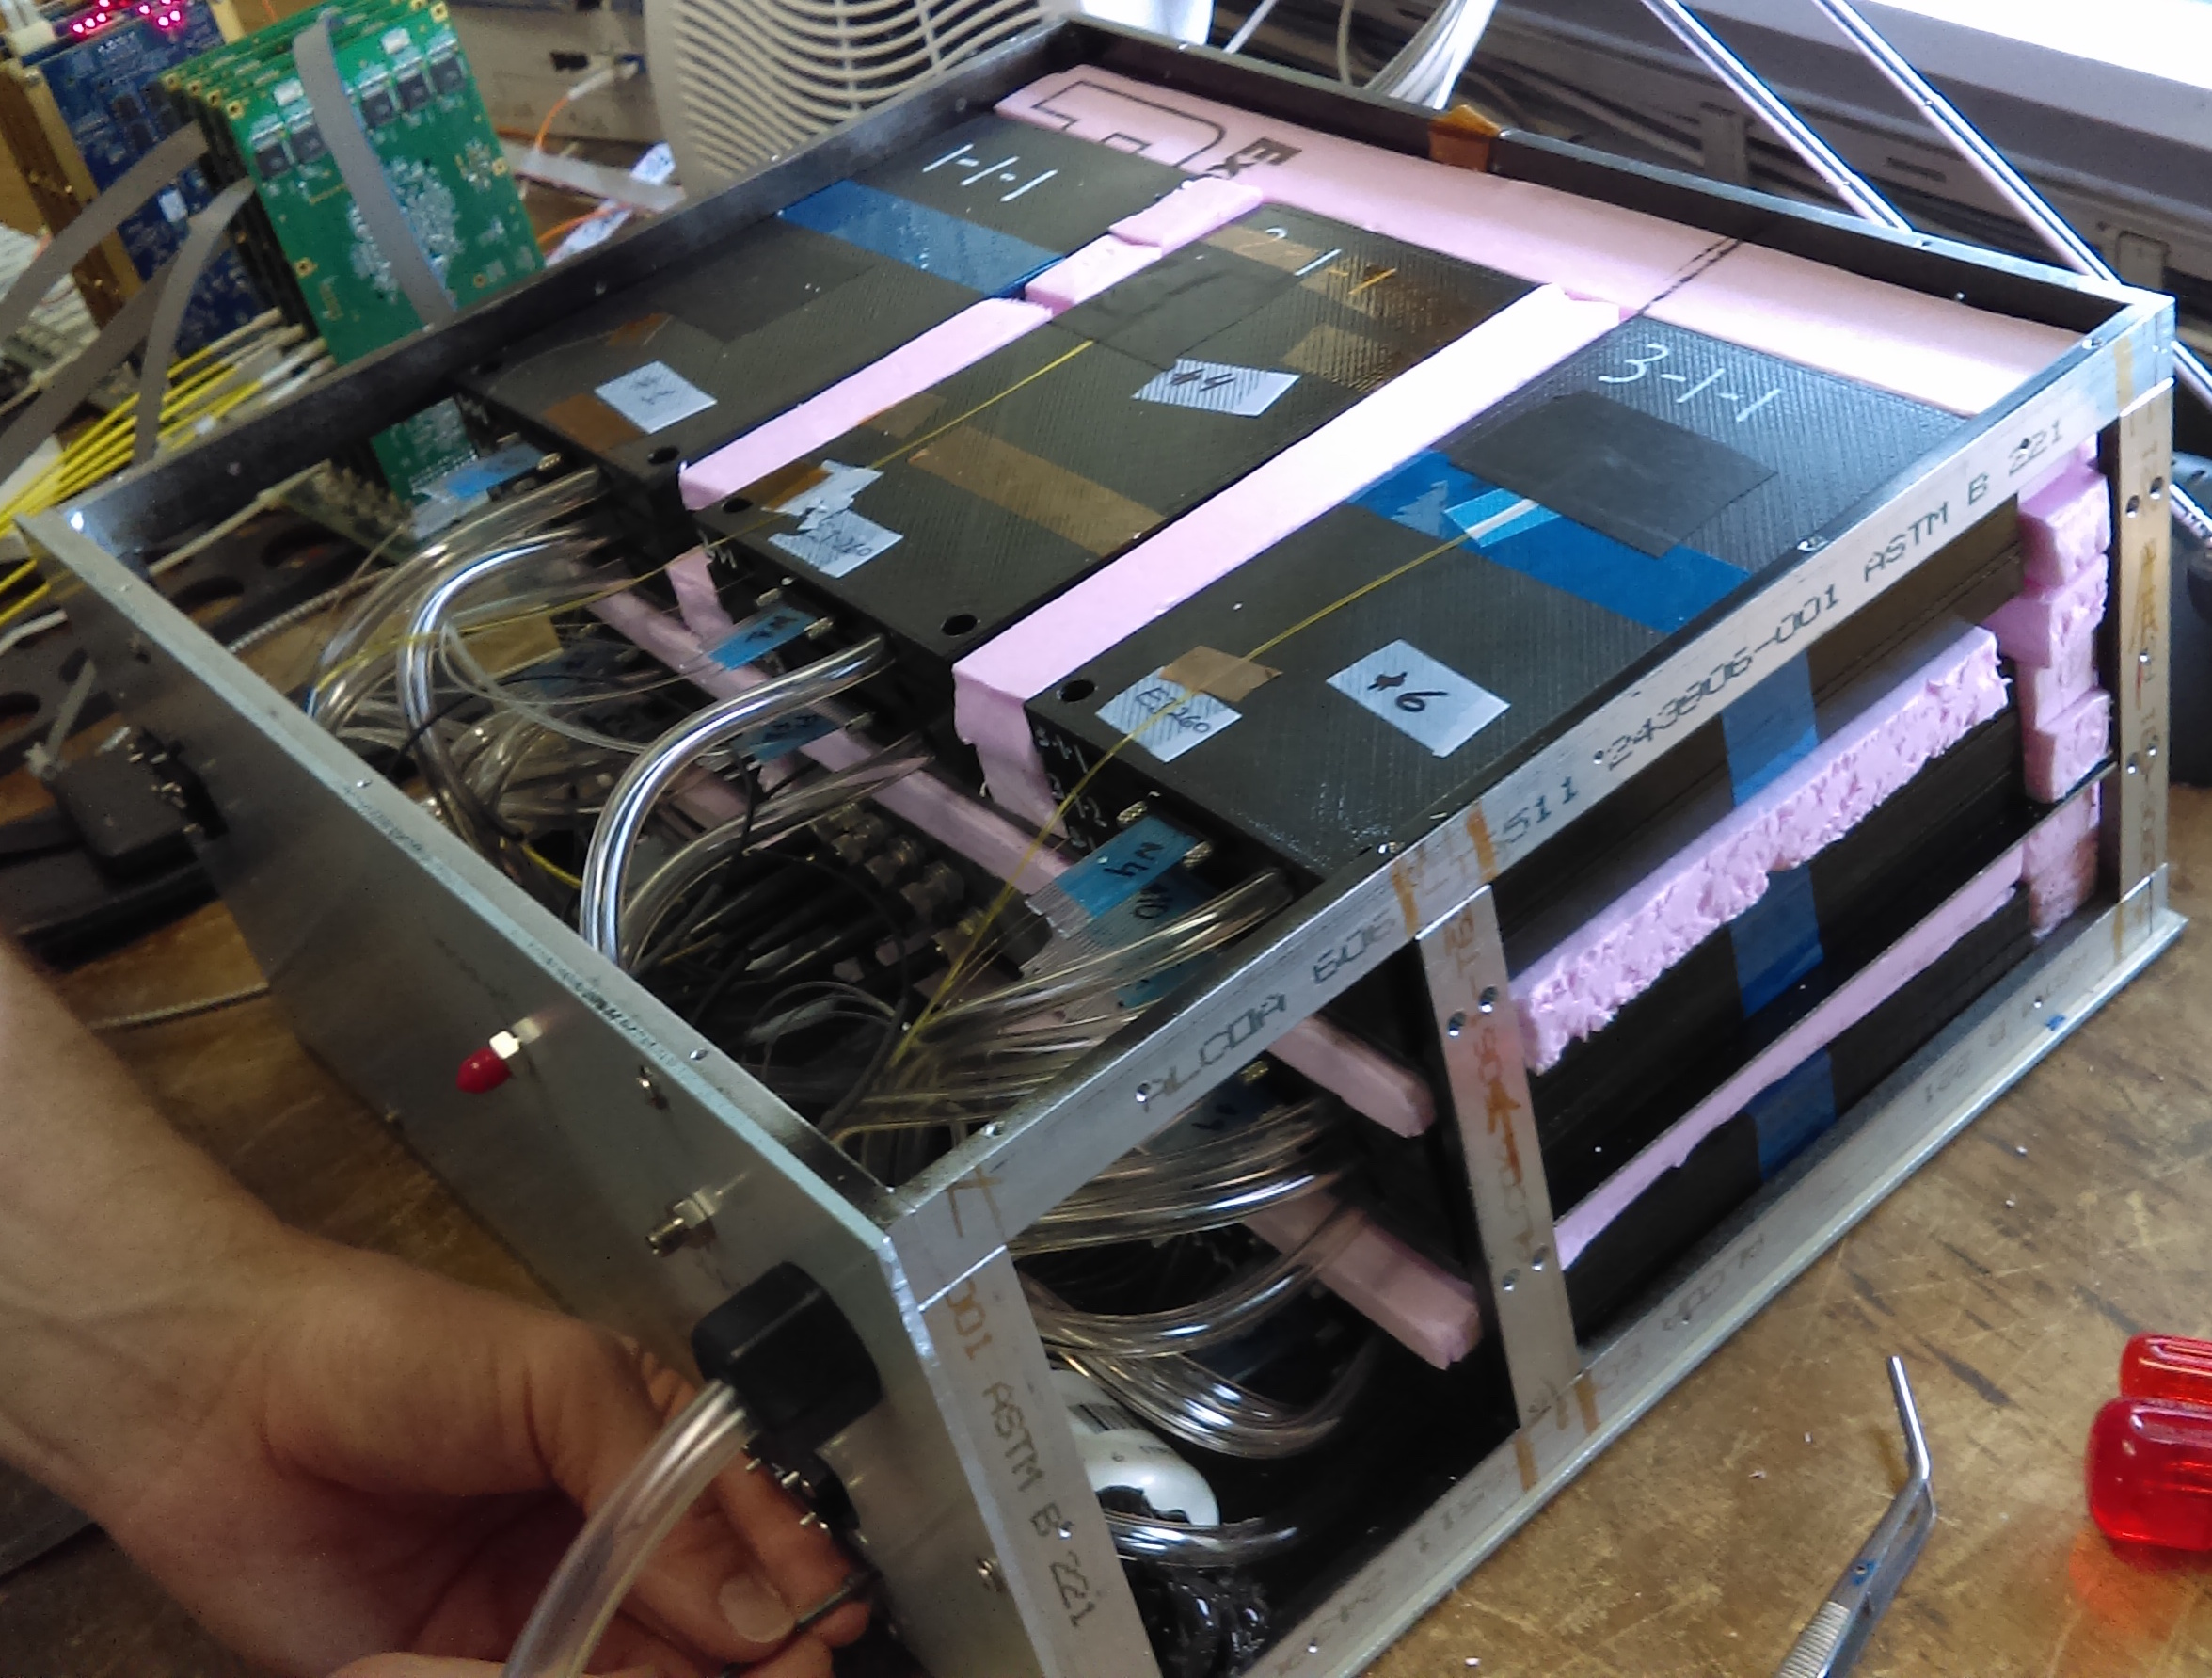
\includegraphics[width=0.8\textwidth]{figures/dark-box-1}
\caption{Photo of a partially disassembled Dark Box with some of the walls removed. Inside the Dark Box are: an array of 24 scintillator cassettes (black plastic boxes), a laser splitter box, cables of clear fibers, a dry air distribution system, and pieces of styrofoam that hold the cassettes in position.}
\label{fig:dark-box-1}
\end{center}
\end{figure}

\begin{figure}[hbtp]
\begin{center}
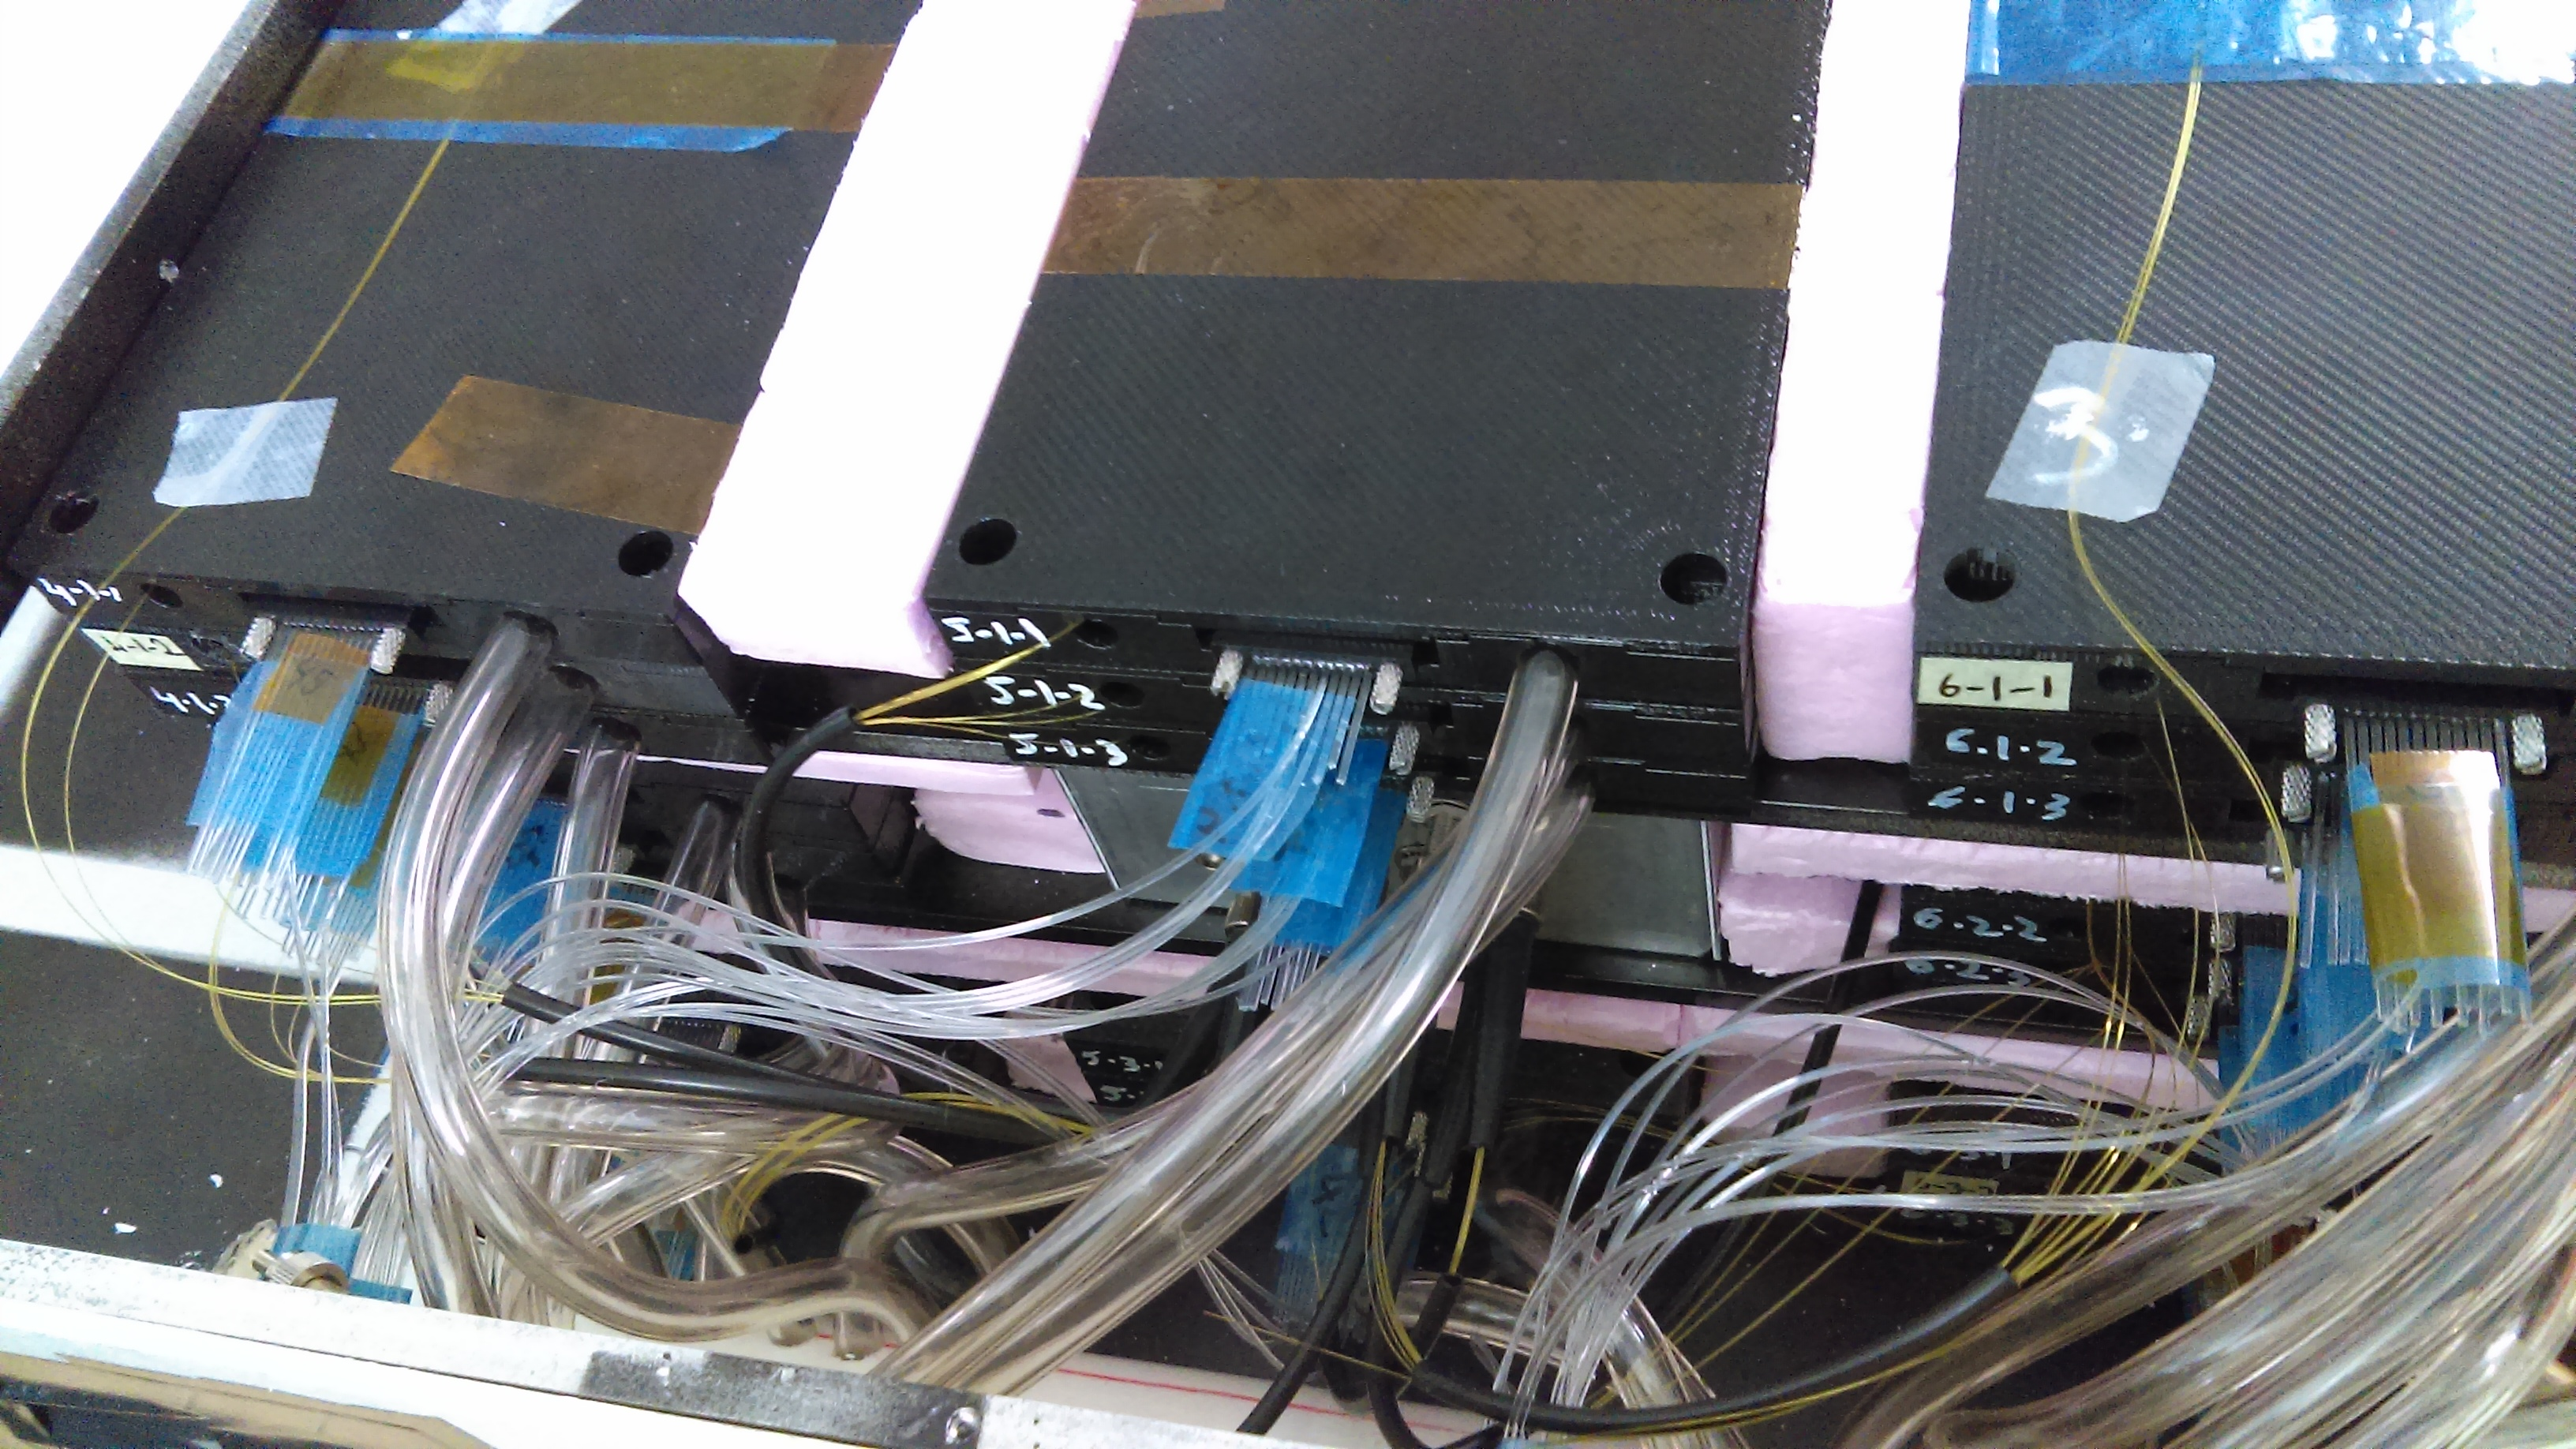
\includegraphics[width=0.8\textwidth]{figures/dark-box-2}
\caption{Zoomed-in view of the interior of a Dark Box. A cluster of clear fibers (reinforced by blue tape) interfaces with the output connector of each cassette. The laser input fibers are thin and yellow in colour; extra, unused laser fibers can be seen taped to the top wall of some cassettes. Thick transparent plastic tubes distribute dry air into the cassettes.}
\label{fig:dark-box-2}
\end{center}
\end{figure}

\subsection{Signal readout\label{sec:setup-readout}}
The clear fibers coming from the Dark Boxes are connected to Phase I HE readout modules (RMs) that receive the scintillation light carried by the clear fibers. The RMs used in this study have a special 1-to-1 optical decoding unit design, meaning that each incoming clear fiber shines onto one unique SiPM inside the RM. Thus, each individual tile (sigma, finger, or other) is read out by a single SiPM channel in an RM. Two RMs are used in the readout, one for each Dark Box; the RM dedicated to Dark Box 1 is referred to as RM1, and RM2 reads out Dark Box 2. Each RM has a total of 48 readout channels. The bias voltages of the SiPMs have been calibrated so that the gain is 47.44 fC with a standard deviation of 2.1\% (see Figure~\ref{fig:gaindist}).

\begin{figure}[hbtp]
\begin{center}
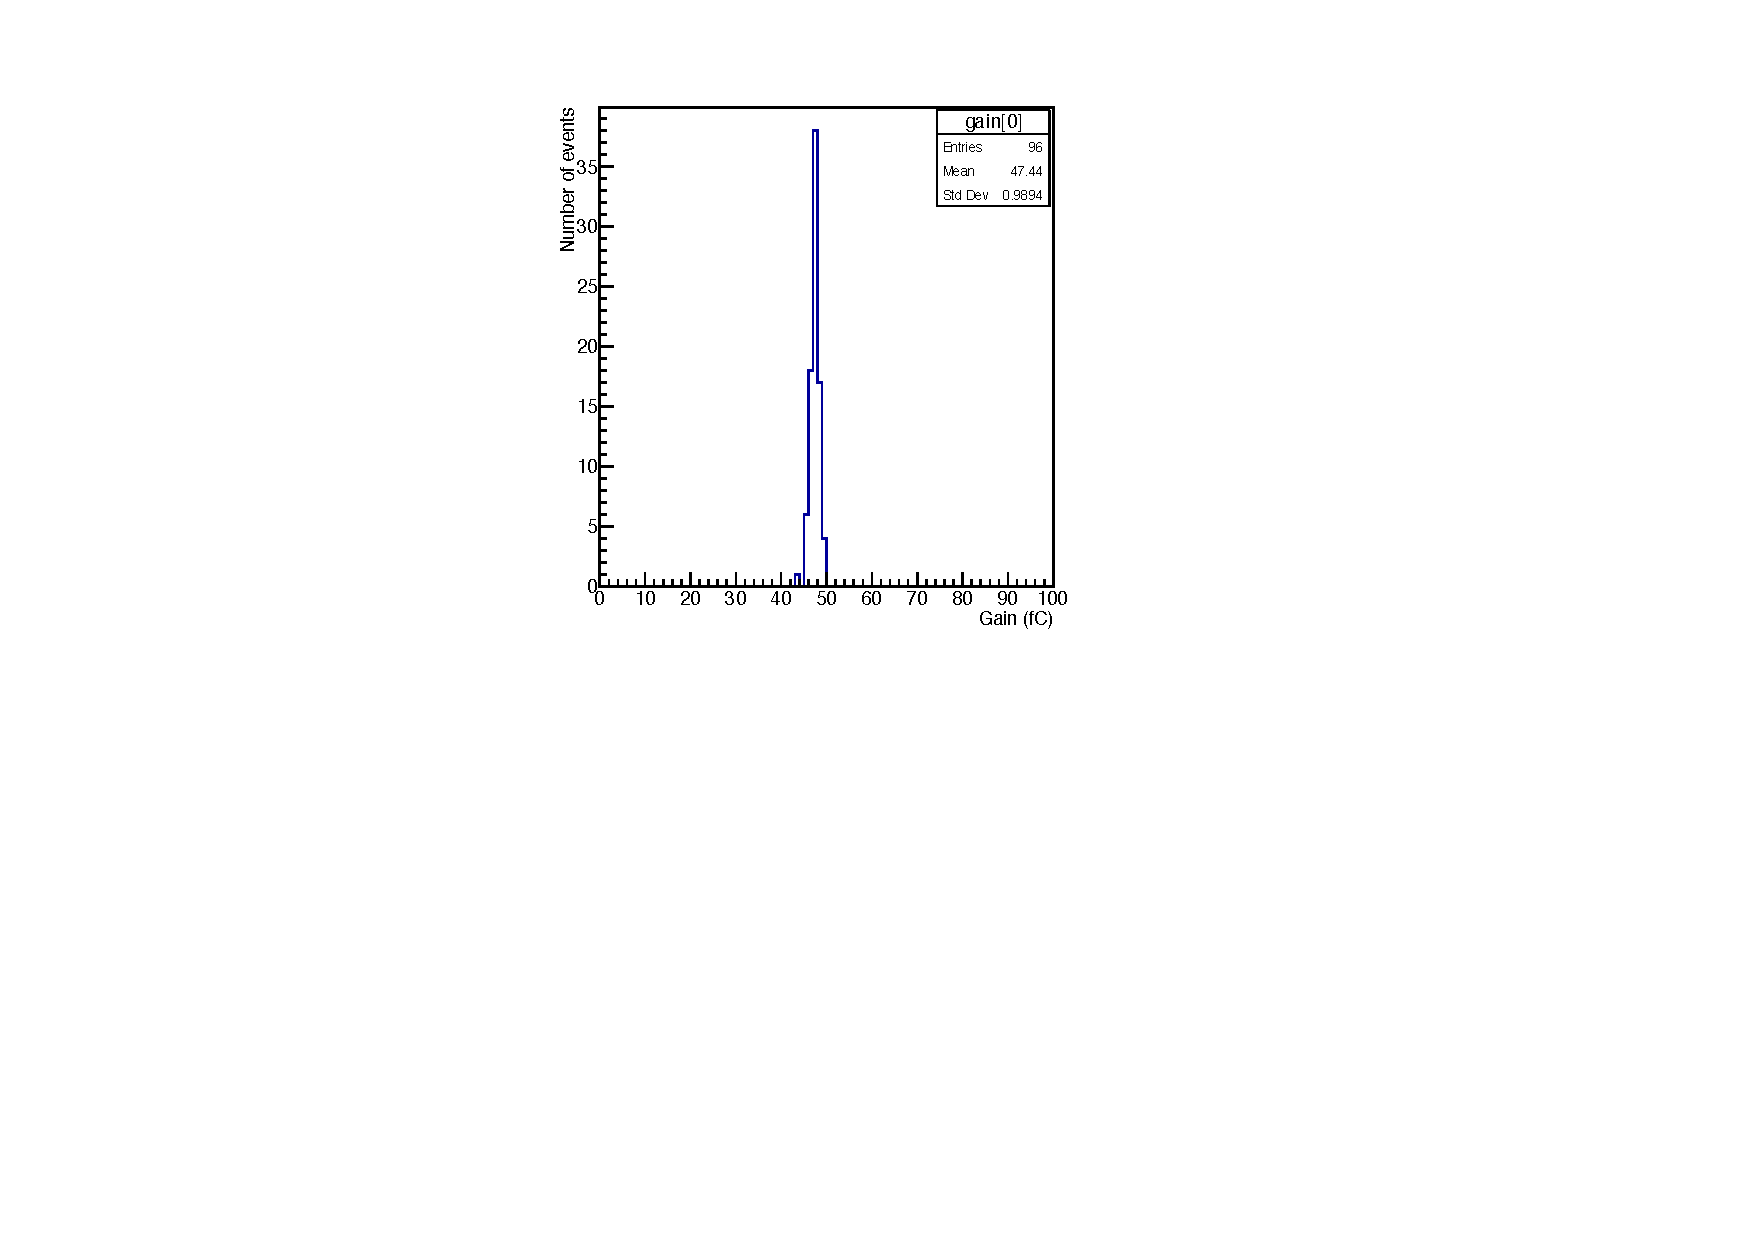
\includegraphics[width=0.8\textwidth]{figures/Run280646_RM1and2_Gains}
\caption{Gain distribution for all channels of RMs 1 and 2 combined (a total of 96 channels) at the start of data-taking with the CRF setup.}
\label{fig:gaindist}
\end{center}
\end{figure}

Charge-integrating QIE11 ADCs digitize the SiPM analog signals, which are then received by a microTCA HCAL Trigger and Readout ($\mu$HTR) card. A new generation Clock and Control Module (ngCCM) controls the CRF front-end. In addition to studying the radiation tolerance properties of upgrade scintillator material candidates, this experiment also serves as a trial run of these Phase I HE front-end and back-end electronics in the experimental cavern.

\subsection{Reference tiles\label{sec:setup-reftiles}}

Throughout the duration of the experiment, the laser amplitude changed dramatically from run to run, due to depletion and refilling of the laser gas. This variation in the measured signal from the tiles from run to run has been taken into account through the use of a reference tile, located outside of CRF and not exposed to a significant dose, but otherwise sharing the same laser and readout pathways as the other channels. In every run, the signal measured in each tile would be normalized to the reference tile signal, thus cancelling out the signal amplitude fluctuation due to the status of the laser gas.

Two reference tiles were used in this experiment. They were located in the TOTEM rack, where the CRF readout box containing the RMs was held. However, the amount of radiation in tis zone was not correctly estimated before the start of the experiment and was actually an order of magnitude higher than expected, reaching a fluence of roughly 1-2$\cdot10^{10}$ neutrons/cm$^{2}$. This caused two important complications. The first was that the SiPMs were damaged by the radiation, and their single photoelectron spectra were progressively drowned by increasing dark current. The second was one of the reference tiles received a significant amount of damage, as evidenced by an exponential decay in its light yield in comparison with the other tile during the irradiation period.

Due to the lack of distinguishable photoelectron peaks after the first 2.3 fb$^{-1}$ of integrated luminosity, the SiPM gain for each subsequent run could not be calculated from the position of the pedestal and first photoelectron peak. However, an alternate method of measuring the gain was developed, and the gain was shown to be reasonably stable during the irradiation period. The damage to one of the reference tiles meant that it could not be relied upon to normalize the light yield of the CRF tiles. Thus, all the tiles were normalized to the signal from the other, less-damaged reference tile.
